%  A simple AAU report template.
%  2015-05-08 v. 1.2.0
%  Copyright 2010-2015 by Jesper Kjær Nielsen <jkn@es.aau.dk>
%
%  This is free software: you can redistribute it and/or modify
%  it under the terms of the GNU General Public License as published by
%  the Free Software Foundation, either version 3 of the License, or
%  (at your option) any later version.
%
%  This is distributed in the hope that it will be useful,
%  but WITHOUT ANY WARRANTY; without even the implied warranty of
%  MERCHANTABILITY or FITNESS FOR A PARTICULAR PURPOSE.  See the
%  GNU General Public License for more details.
%
%  You can find the GNU General Public License at <http://www.gnu.org/licenses/>.
%
%  A simple AAU report template.
%  2015-05-08 v. 1.2.0
%  Copyright 2010-2015 by Jesper Kjær Nielsen <jkn@es.aau.dk>
%
%  This is free software: you can redistribute it and/or modify
%  it under the terms of the GNU General Public License as published by
%  the Free Software Foundation, either version 3 of the License, or
%  (at your option) any later version.
%
%  This is distributed in the hope that it will be useful,
%  but WITHOUT ANY WARRANTY; without even the implied warranty of
%  MERCHANTABILITY or FITNESS FOR A PARTICULAR PURPOSE.  See the
%  GNU General Public License for more details.
%
%  You can find the GNU General Public License at <http://www.gnu.org/licenses/>.
%
\documentclass[11pt,twoside,a4paper,openright]{report}
%%%%%%%%%%%%%%%%%%%%%%%%%%%%%%%%%%%%%%%%%%%%%%%%
% Language, Encoding and Fonts
% http://en.wikibooks.org/wiki/LaTeX/Internationalization
%%%%%%%%%%%%%%%%%%%%%%%%%%%%%%%%%%%%%%%%%%%%%%%%
% Select encoding of your inputs. Depends on
% your operating system and its default input
% encoding. Typically, you should use
%   Linux  : utf8 (most modern Linux distributions)
%            latin1
%   Windows: ansinew
%            latin1 (works in most cases)
%   Mac    : applemac
% Notice that you can manually change the input
% encoding of your files by selecting "save as"
% an select the desired input encoding.
\usepackage[utf8]{inputenc}
% Make latex understand and use the typographic
% rules of the language used in the document.
\usepackage[danish,english]{babel}
% Use the palatino font
\usepackage[sc]{mathpazo}
\linespread{1.05}         % Palatino needs more leading (space between lines)
% Choose the font encoding
\usepackage[T1]{fontenc}
%%%%%%%%%%%%%%%%%%%%%%%%%%%%%%%%%%%%%%%%%%%%%%%%
% Graphics and Tables
% http://en.wikibooks.org/wiki/LaTeX/Importing_Graphics
% http://en.wikibooks.org/wiki/LaTeX/Tables
% http://en.wikibooks.org/wiki/LaTeX/Colors
%%%%%%%%%%%%%%%%%%%%%%%%%%%%%%%%%%%%%%%%%%%%%%%%
% load a colour package
\usepackage{xcolor}
\definecolor{aaublue}{RGB}{33,26,82}% dark blue
% The standard graphics inclusion package
\usepackage{graphicx}
% Set up how figure and table captions are displayed
\usepackage{caption}
\captionsetup{%
  font=footnotesize,% set font size to footnotesize
  labelfont=bf % bold label (e.g., Figure 3.2) font
}
% Make the standard latex tables look so much better
\usepackage{array,booktabs}
% Enable the use of frames around, e.g., theorems
% The framed package is used in the example environment
\usepackage{framed}

%%%%%%%%%%%%%%%%%%%%%%%%%%%%%%%%%%%%%%%%%%%%%%%%
% Mathematics
% http://en.wikibooks.org/wiki/LaTeX/Mathematics
%%%%%%%%%%%%%%%%%%%%%%%%%%%%%%%%%%%%%%%%%%%%%%%%
% Defines new environments such as equation,
% align and split
\usepackage{amsmath}
% Adds new math symbols
\usepackage{amssymb}
% Use theorems in your document
% The ntheorem package is also used for the example environment
% When using thmmarks, amsmath must be an option as well. Otherwise \eqref doesn't work anymore.
\usepackage[framed,amsmath,thmmarks]{ntheorem}

%%%%%%%%%%%%%%%%%%%%%%%%%%%%%%%%%%%%%%%%%%%%%%%%
% Page Layout
% http://en.wikibooks.org/wiki/LaTeX/Page_Layout
%%%%%%%%%%%%%%%%%%%%%%%%%%%%%%%%%%%%%%%%%%%%%%%%
% Change margins, papersize, etc of the document
\usepackage[
  inner=28mm,% left margin on an odd page
  outer=41mm,% right margin on an odd page
  ]{geometry}
% Modify how \chapter, \section, etc. look
% The titlesec package is very configureable
\usepackage{titlesec}
\titleformat{\chapter}[display]{\normalfont\huge\bfseries}{\chaptertitlename\ \thechapter}{20pt}{\Huge}
\titleformat*{\section}{\normalfont\Large\bfseries}
\titleformat*{\subsection}{\normalfont\large\bfseries}
\titleformat*{\subsubsection}{\normalfont\normalsize\bfseries}
%\titleformat*{\paragraph}{\normalfont\normalsize\bfseries}
%\titleformat*{\subparagraph}{\normalfont\normalsize\bfseries}

% Clear empty pages between chapters
\let\origdoublepage\cleardoublepage
\newcommand{\clearemptydoublepage}{%
  \clearpage
  {\pagestyle{empty}\origdoublepage}%
}
\let\cleardoublepage\clearemptydoublepage

% Change the headers and footers
\usepackage{fancyhdr}
\pagestyle{fancy}
\fancyhf{} %delete everything
\renewcommand{\headrulewidth}{0pt} %remove the horizontal line in the header
\fancyhead[RE]{\small\nouppercase\leftmark} %even page - chapter title
\fancyhead[LO]{\small\nouppercase\rightmark} %uneven page - section title
\fancyhead[LE,RO]{\thepage} %page number on all pages
% Do not stretch the content of a page. Instead,
% insert white space at the bottom of the page
\raggedbottom
% Enable arithmetics with length. Useful when
% typesetting the layout.
\usepackage{calc}

%%%%%%%%%%%%%%%%%%%%%%%%%%%%%%%%%%%%%%%%%%%%%%%%
% Bibliography
% http://en.wikibooks.org/wiki/LaTeX/Bibliography_Management
%%%%%%%%%%%%%%%%%%%%%%%%%%%%%%%%%%%%%%%%%%%%%%%%
\usepackage[backend=bibtex,
  bibencoding=utf8
  ]{biblatex}
\addbibresource{bib/mybib}

%%%%%%%%%%%%%%%%%%%%%%%%%%%%%%%%%%%%%%%%%%%%%%%%
% Misc
%%%%%%%%%%%%%%%%%%%%%%%%%%%%%%%%%%%%%%%%%%%%%%%%
% Add bibliography and index to the table of
% contents
\usepackage[nottoc]{tocbibind}
% Add the command \pageref{LastPage} which refers to the
% page number of the last page
\usepackage{lastpage}
% Add todo notes in the margin of the document
\usepackage[
%  disable, %turn off todonotes
  colorinlistoftodos, %enable a coloured square in the list of todos
  textwidth=\marginparwidth, %set the width of the todonotes
  textsize=scriptsize, %size of the text in the todonotes
  ]{todonotes}

%%%%%%%%%%%%%%%%%%%%%%%%%%%%%%%%%%%%%%%%%%%%%%%%
% Hyperlinks
% http://en.wikibooks.org/wiki/LaTeX/Hyperlinks
%%%%%%%%%%%%%%%%%%%%%%%%%%%%%%%%%%%%%%%%%%%%%%%%
% Enable hyperlinks and insert info into the pdf
% file. Hypperref should be loaded as one of the
% last packages
\usepackage{hyperref}
\hypersetup{%
	pdfpagelabels=true,%
	plainpages=false,%
	pdfauthor={Author(s)},%
	pdftitle={Title},%
	pdfsubject={Subject},%
	bookmarksnumbered=true,%
	colorlinks=true,%
	citecolor=black,%
	filecolor=black,%
	linkcolor=black,% you should probably change this to black before printing
	urlcolor=black,%
	pdfstartview=FitH%
}

\usepackage{cleveref}
\usepackage{relsize}

\usepackage[lined,boxed,commentsnumbered,linesnumbered]{algorithm2e}

\usepackage{mathtools}
% package inclusion and set up of the document
\input{setup/hyphenations.tex}%
%  A simple AAU report template.
%  2015-05-08 v. 1.2.0
%  Copyright 2010-2015 by Jesper Kjær Nielsen <jkn@es.aau.dk>
%
%  This is free software: you can redistribute it and/or modify
%  it under the terms of the GNU General Public License as published by
%  the Free Software Foundation, either version 3 of the License, or
%  (at your option) any later version.
%
%  This is distributed in the hope that it will be useful,
%  but WITHOUT ANY WARRANTY; without even the implied warranty of
%  MERCHANTABILITY or FITNESS FOR A PARTICULAR PURPOSE.  See the
%  GNU General Public License for more details.
%
%  You can find the GNU General Public License at <http://www.gnu.org/licenses/>.
%
%
%
% see, e.g., http://en.wikibooks.org/wiki/LaTeX/Customizing_LaTeX#New_commands
% for more information on how to create macros

%%%%%%%%%%%%%%%%%%%%%%%%%%%%%%%%%%%%%%%%%%%%%%%%
% Macros for the titlepage
%%%%%%%%%%%%%%%%%%%%%%%%%%%%%%%%%%%%%%%%%%%%%%%%
%Creates the aau titlepage
\newcommand{\aautitlepage}[3]{%
  {
    %set up various length
    \ifx\titlepageleftcolumnwidth\undefined
      \newlength{\titlepageleftcolumnwidth}
      \newlength{\titlepagerightcolumnwidth}
    \fi
    \setlength{\titlepageleftcolumnwidth}{0.5\textwidth-\tabcolsep}
    \setlength{\titlepagerightcolumnwidth}{\textwidth-2\tabcolsep-\titlepageleftcolumnwidth}
    %create title page
    \thispagestyle{empty}
    \noindent%
    \begin{tabular}{@{}ll@{}}
      \parbox{\titlepageleftcolumnwidth}{
        \iflanguage{danish}{%
          \includegraphics[width=\titlepageleftcolumnwidth]{figures/aau_logo_da}
        }{%
          \includegraphics[width=\titlepageleftcolumnwidth]{figures/aau_logo_en}
        }
      } &
      \parbox{\titlepagerightcolumnwidth}{\raggedleft\sf\small
        #2
      }\bigskip\\
       #1 &
      \parbox[t]{\titlepagerightcolumnwidth}{%
      \textbf{Abstract:}\bigskip\par
        \fbox{\parbox{\titlepagerightcolumnwidth-2\fboxsep-2\fboxrule}{%
          #3
        }}
      }\\
    \end{tabular}
    \vfill
    \iflanguage{danish}{%
      \noindent{\footnotesize\emph{Rapportens indhold er frit tilgængeligt, men offentliggørelse (med kildeangivelse) må kun ske efter aftale med forfatterne.}}
    }{%
      \noindent{\footnotesize\emph{The content of this report is freely available, but publication (with reference) may only be pursued due to agreement with the author.}}
    }
    \clearpage
  }
}

%Create english project info
\newcommand{\englishprojectinfo}[8]{%
  \parbox[t]{\titlepageleftcolumnwidth}{
    \textbf{Title:}\\ #1\bigskip\par
    \textbf{Theme:}\\ #2\bigskip\par
    \textbf{Project Period:}\\ #3\bigskip\par
    \textbf{Project Group:}\\ #4\bigskip\par
    \textbf{Participant(s):}\\ #5\bigskip\par
    \textbf{Supervisor(s):}\\ #6\bigskip\par
    \textbf{Copies:} #7\bigskip\par
    \textbf{Page Numbers:} \pageref{LastPage}\bigskip\par
    \textbf{Date of Completion:}\\ #8
  }
}

%Create danish project info
\newcommand{\danishprojectinfo}[8]{%
  \parbox[t]{\titlepageleftcolumnwidth}{
    \textbf{Titel:}\\ #1\bigskip\par
    \textbf{Tema:}\\ #2\bigskip\par
    \textbf{Projektperiode:}\\ #3\bigskip\par
    \textbf{Projektgruppe:}\\ #4\bigskip\par
    \textbf{Deltager(e):}\\ #5\bigskip\par
    \textbf{Vejleder(e):}\\ #6\bigskip\par
    \textbf{Oplagstal:} #7\bigskip\par
    \textbf{Sidetal:} \pageref{LastPage}\bigskip\par
    \textbf{Afleveringsdato:}\\ #8
  }
}
% my new macros
\newcounter{todofull}

%\newcommand*\rfrac[2]{\ensuremath{{}^{#1}\!/_{#2}}}
%\newcommand*\rfrac[2]{\fbox{\ensuremath{\frac{#1}{#2}}}}
\newcommand*\rfrac[2]{{\scriptsize #1|#2}\space}

\newcommand{\namedtodo}[5]
{
  \stepcounter{todofull}
  \ifthenelse{\equal{#1}{}}
  {
    \todo[backgroundcolor=#4,linecolor=#4,caption=
    {\textbf{\arabic{todofull} #3: } #2}]
    {\color{#5}\textbf{\arabic{todofull} #3: }#2}
  }
  {
    \todo[backgroundcolor=#4,linecolor=#4,caption=
    {\textbf{\arabic{todofull} #3: } #1}]
    {\color{#5}\textbf{\arabic{todofull} #3: }#2}
  }
}
\newcommand{\namedtodoinline}[5]
{
  \stepcounter{todofull}
  \ifthenelse{\equal{#1}{}}
  {
    \todo[backgroundcolor=#4,inline,caption=
    {\textbf{\arabic{todofull} #3: } #2}]
    {\normalsize\color{#5}\textbf{\arabic{todofull} #3: }#2}
  }
  {
    \todo[backgroundcolor=#4,inline,caption=
    {\textbf{\arabic{todofull} #3: } #1}]
    {\normalsize\color{#5}\textbf{\arabic{todofull} #3: }#2}
  }
}
\newcommand{\mikkel}[2][]
{
  \namedtodo{#1}{#2}
  {Mikkel}{blue!80}{white}
}
\newcommand{\mikkelin}[2][]
{
  \namedtodoinline{#1}{#2}
  {Mikkel}{blue!80}{white}
}
\newcommand{\mikael}[2][]
{
  \namedtodo{#1}{#2}
  {Mikael}{green}{black}
}
\newcommand{\mikaelin}[2][]
{
  \namedtodoinline{#1}{#2}
  {Mikael}{green}{black}
}
\newcommand{\rene}[2][]
{
  \namedtodo{#1}{#2}
  {René}{purple}{white}
}
\newcommand{\renein}[2][]
{
  \namedtodoinline{#1}{#2}
  {René}{purple}{white}
}

\newcommand{\mads}[2][]
{
  \namedtodoinline{#1}{#2}
  {Mads}{yellow}{red}
}

\makeatletter \renewcommand \listoftodos{\section*{List of Todos} \@starttoc{tdo}}
% personal todo note styles
\newcommand{\thetool}{the flow-checking tool}

\newcommand{\thelang}{CTIF}
\newcommand{\thelanglong}{C Timed Information Flow}
% commands used for changeable aliases
\usepackage{listings}

\newcommand{\dlmcsyntax}[1]{\color{violet}{#1}}

\lstdefinestyle{dlmc}{
  belowcaptionskip=1\baselineskip,
  breaklines=true,
  captionpos=b,
  xleftmargin=\parindent,
  language=C,
  showstringspaces=false,
  morekeywords={bool, user\_info},
  basicstyle=\ttfamily,
  keywordstyle=\bfseries\color{blue},
  commentstyle=\itshape\color{green!50!black},
  stringstyle=\color{red!50!black},
  mathescape=true,%
  columns=fullflexible,
  keepspaces,
  escapeinside={(*@}{@*)},
  morekeywords=[2]{principal,this,caller},
  keywordstyle=[2]\dlmcsyntax,
  keywordstyle=[3]\dlmcsyntax,
  moredelim = [s][\dlmcsyntax]{\{\{}{\}\}},
  literate= {-->?}{{\dlmcsyntax{-{}->?}}}1
            {<|}{{\dlmcsyntax{<|}}}1
            {|>}{{\dlmcsyntax{|>}}}1
            {@}{{\dlmcsyntax{@}}}1
            {@?}{{\dlmcsyntax{@?}}}1
}

\newcommand{\dlmc}[1]{\lstinline[style=dlmc]{#1}}
% source code listings
\theoremheaderfont{\normalfont\bfseries}
\theorembodyfont{\normalfont}
\theoremstyle{break}
\def\theoremframecommand{{\color{gray!50}\vrule width 5pt \hspace{5pt}}}
\newshadedtheorem{exa}{Example}[chapter]
\newenvironment{example}[1]{%
		\begin{exa}[#1]
}{%
		\end{exa}
}

\newshadedtheorem{defini}{Definition}[chapter]
\newenvironment{definition}[1]{%
    \begin{defini}[#1]
}{%
    \end{defini}
}

\newcommand{\gp}{\; | \;} % extra margin grammar pipe
\newcommand{\tk}[1]{\, \texttt{#1} \,} % token style
\newcommand{\argpart}[3]{ % IN, ARROW-NAME, OUT
	\langle #1 \rangle \rightarrow_{#2} #3}
\newcommand{\vlbl}[1]{\underline{#1}} % variable label
\newcommand{\clbl}[1]{\overline{#1}} % constant label

\newcommand{\iVar}{\mathbf{Var}}
\newcommand{\iFun}{\mathbf{Fun}}
\newcommand{\iDecv}{\mathbf{DecV}}
\newcommand{\iDecf}{\mathbf{DecF}}
\newcommand{\iDecp}{\mathbf{DecP}}
\newcommand{\iStmc}{\mathbf{StmC}}
\newcommand{\iExp}{\mathbf{Exp}}
\newcommand{\iExpl}{\mathbf{ExpL}}
\newcommand{\iLbl}{\mathbf{Lbl}}
\newcommand{\iStm}{\mathbf{Stm}}
\newcommand{\iProg}{\mathbf{Prog}}
\newcommand{\iCstr}{\mathbf{Cstr}}
\newcommand{\iStml}{\mathbf{StmL}}
\newcommand{\iPrin}{\mathbf{Prin}}
\newcommand{\ia}{\alpha} % authority label
\newcommand{\ib}{\beta} % block label
\newcommand{\ifb}{\phi} % function block label

\newcommand{\truleHelper}[4]{
	\text{[#1]} \hspace{2em}  & \ifthenelse{\equal{#3}{}}{#2}{\frac{#3}{#2}} \nonumber \\[1em]
														& \parbox{\textwidth}{#4} \nonumber
}

\newcommand{\trule}[4]{% NAME, CONCLUSION, PREMISES, SIDE CONDITIONS
\begin{align}
  \truleHelper{#1}{#2}{#3}{#4}
\end{align}}

\newenvironment{trules}{%
	\renewcommand{\trule}[4]{\truleHelper{##1}{##2}{##3}{##4} \\[1em] \nonumber}
  \align%
}{%
  \endalign%
}

\DeclareMathOperator*{\sqcupl}{\mathlarger{\mathlarger\sqcup}}
% math commands

\begin{document}
\usetikzlibrary{arrows}
%frontmatter
\pagestyle{empty} %disable headers and footers
\listoftodos
\clearpage
\pagenumbering{roman} %use roman page numbering in the frontmatter
%  A simple AAU report template.
%  2015-05-08 v. 1.2.0
%  Copyright 2010-2015 by Jesper Kjær Nielsen <jkn@es.aau.dk>
%
%  This is free software: you can redistribute it and/or modify
%  it under the terms of the GNU General Public License as published by
%  the Free Software Foundation, either version 3 of the License, or
%  (at your option) any later version.
%
%  This is distributed in the hope that it will be useful,
%  but WITHOUT ANY WARRANTY; without even the implied warranty of
%  MERCHANTABILITY or FITNESS FOR A PARTICULAR PURPOSE.  See the
%  GNU General Public License for more details.
%
%  You can find the GNU General Public License at <http://www.gnu.org/licenses/>.
%
\pdfbookmark[0]{Front page}{label:frontpage}%
\begin{titlepage}
  \addtolength{\hoffset}{0.5\evensidemargin-0.5\oddsidemargin} %set equal margins on the frontpage - remove this line if you want default margins
  \noindent%
  \begin{tabular}{@{}p{\textwidth}@{}}
    \toprule[2pt]
    \midrule
    \vspace{0.2cm}
    \begin{center}
    \Huge{\textbf{
      C Timed Information Flow% insert your title here
    }}
    \end{center}
    \begin{center}
      \Large{
        - A Practical Approach -% insert your subtitle here
      }
    \end{center}
    \vspace{0.2cm}\\
    \midrule
    \toprule[2pt]
  \end{tabular}
  \vspace{4 cm}
  \begin{center}
    {\large
      Master's Thesis%Insert document type (e.g., Project Report)
    }\\
    \vspace{0.2cm}
    {\Large
      DES105F16%Insert your group name or real names here
    }
  \end{center}
  \vfill
  \begin{center}
  Aalborg University\\
  Department of Computer Science
  \end{center}
\end{titlepage}
\clearpage

\thispagestyle{empty}
{\small
\strut\vfill % push the content to the bottom of the page
\noindent Copyright \copyright{} Aalborg University 2016\par
\clearpage

% !TEX root = ../master.tex
\pdfbookmark[0]{English title page}{label:titlepage_en}
\aautitlepage{%
  \englishprojectinfo{
    C Timed Information Flow% \\
    %-- A Practical Approach%title
  }{%
    IoT Security %theme
  }{%
    Spring Semester 2016 %project period
  }{%
    DES105F16 % project group
  }{%
    %list of group members
    Mikael Elkiær Christensen\\
    Mikkel Sandø Larsen
  }{%
    %list of supervisors
    René Rydhof Hansen\\
    Mads Chr. Olesen
  }{%
    2 % number of printed copies
  }{%
    \today % date of completion
  }{%
    \url{https://github.com/des105f16/Editor/tree/d074ede4d55c6565b9d6eac651e24dff32d754cf}
  }%
}{%department and address
  \textbf{Department of Computer Science}\\
  Aalborg University\\
  \href{http://cs.aau.dk}{http://cs.aau.dk}
}{% the abstract
  This report describes the tool \thelanglong{} (\thelang), which can take new and existing C source code, allowing for labeling of security policies applied directly to the source.
  The tool can then, based on the labeling, provide feedback about any potential breaches of security as labeled information flows through the program.

  These security policy labels are based on \emph{The Decentralized Label Model} (DLM).
  The report takes important concepts of DLM and provides an extended description as well as a formalization in regards to the inferrence of security policy labels.
  Additionally, an extension to the security policies are provided, by allowing the expression of time policies, which similarly will be checked by the tool.
  These time policies were created with a focus on their simplicity and practical applications in mind.

  As a first step in formalizing the time policy extension, it will be shown how they can be translated into \emph{timed automata}.
  In order to ascertain the practical applications, the time policies will be compared with \emph{The Timed Decentralized Label Model}, which takes a more theoretical approach.
}

\cleardoublepage
\pdfbookmark[0]{Contents}{label:contents}
\pagestyle{fancy} %enable headers and footers again
\tableofcontents
% !TEX root = ../master.tex
\chapter*{Summary\markboth{Summary}{Summary}}\label{ch:summary}
\addcontentsline{toc}{chapter}{Summary}

This report represents the project \thelanglong{} (\thelang), which resulted in a tool of the same name.
The \thelang{} tool allows for writing C programs, with the ability to express security policies in order to ensure information flow.
These security policies are based upon those of \emph{The Decentralized Label Model} (DLM), with a focus on making its use as seamless as possible, by allowing for sophisticated inferrence.
Further, these security policies are extended with the ability to express simple and powerful time policies.

The project provides two main contributions.
Firstly, formalizations of important DLM concepts are provided.
Especially those concepts related to label inferrence, and constraint checking -- the main driver of inferrence, have been formalized by providing an extended description, as well as a denotational semantics.
Secondly, an extension to the DLM security policies has been provided in the form of time policies.
These time policies were created as to have a focus on their practical applications.
However, it is also shown how they can be formalized by being translated into timed automata, as well as a comparison with a related model \emph{The Timed Decentralized Label Model}.

The tool itself was written in C\#, employing the SablePP toolbox to generate the compiler, which allows for easy extensibility.
The use of SablePP allowed us to incrementally extend our C language scope, increasing the practical applications of \thelang{}.
It also allowed for great flexibility in defining both syntax and semantics, allowing for fast prototyping/experimenting.

\thelang{} provides a practical and highly usable way of annotating new and existing C source code, allowing for easy analysis of information flow while requiring only minor extension.
Very few constructs are added to the C syntax, as to not over-complicate its potential uses, while keeping it both highly useful and powerful.
This is true for both the security policies, as well as time policies.

\chapter*{Preface\markboth{Preface}{Preface}}\label{ch:preface}
\addcontentsline{toc}{chapter}{Preface}
Here is the preface. You should put your signatures at the end of the preface.

\vspace{\baselineskip}\hfill Aalborg University, \today
\vfill\noindent
\begin{minipage}[b]{0.45\textwidth}
 \centering
 \rule{\textwidth}{0.5pt}\\
  Mikael Elkiær Christensen\\
 {\footnotesize <michri11@student.aau.dk>}
\end{minipage}
\hfill
\begin{minipage}[b]{0.45\textwidth}
 \centering
 \rule{\textwidth}{0.5pt}\\
  Mikkel Sandø Larsen\\
 {\footnotesize <milars@student.aau.dk>}
\end{minipage}

\cleardoublepage
%mainmatter
\pagenumbering{arabic} %use arabic page numbering in the mainmatter

\chapter{Introduction}\label{introduction}
% !TEX root = ../../master.tex

In this chapter we will present the needed background information which serves as the base for our project.
We will, based on our pre-specialization \cite{prespecialization}, introduce some of the security problems found in the Internet-of-Things (IoT).
Specifically, we will look into privacy issues associated with IoT.
We will also discuss the possibility of handling some of these privacy issues with time-based constraints.
Additionally, we will discuss some problems related to the development of secure software.
Finally, we will present two code examples, which will be used throughout the report, to serve as IoT use-cases.
The following presentation of our solution will be based on these running examples.

% !TEX root = ../../master.tex

\section{Security problems}
In \cite{prespecialization} we investigated problems involving the imminent implementation of smart meters throughout Europe.\mikael{Fodnote kilde fra forspeciale.}
Here we discovered a wide array of problems, ranging from ethical to practical.
One of the more interesting discoveries that we made was the newly acquired problems associated with increasing the availability of a previously physically isolated device.
This is exactly what is going to happen when the current electrical meters are going to be substituted with remotely accessed and controlled smart meters.
It will open up for problems already found in similar devices, which in general is any IoT device.

One of the focuses we had in \cite{prespecialization} was on the privacy issues related to such an exposed device.
We would like to explore this problem further, while coming up with a solution that will aid the programmer in the securing IoT devices.
Many of the security problems associated with privacy could possibly also be minimized by adding the concept of time constraints, which we will also discuss here.

\subsection{Privacy}
With the emergence of IoT, more and more of our devices are being globally exposed, for both good and for worse.
There will be endless possibilities in easing our everyday lives, both at a personal level and at a communal level.
At the personal level, we will be able to access devices that monitor and control our homes.
On the communal level, many of the tasks that previously had to be done by people can now be pushed to remote devices, such as monitoring the health of patients or changing traffic signs on a freeway.\footnote{\url{http://techcrunch.com/2015/10/24/why-iot-security-is-so-critical/}}

All these things are associated with major potential risks, should they be compromised.
At the personal level, we do not wish to give up any information about our personal lives, and we don't want anyone else controlling our devices.
At the community level the risks can be even larger, especially those devices linked to health care, such as a ``smart'' pacemaker.

Some of these risks are associated with faulty protocols or erroneous implementations of protocols.
However, privacy can still be an issue even with a ``good'' protocol.
The problem here is that it is not easy ensuring that the information managed by an IoT device is distributed as intended.
This is especially true if different policies apply to different users, as is more than likely with IoT devices.
This could for instance be power consumption data which have different policies depending on who is accessing the data, e.g.: the consumer itself, the electrical company, or the hardware manufacturer.
It is also possible to have \emph{passive cheaters}, users of the system who follow the rules, but try to acquire more information than is intended possible.

\subsection{Time constraints}
Properly handling timing within a system is an already-existing and quite common problem.\footnote{\url{http://www.nist.gov/pml/div688/timing-031915.cfm}}
It is something that is hard to both model and ensure that any such modeling holds.
This is especially true for IoT devices which operate in the real world where any potential mistakes can result in great consequence.

To further the concept of protecting privacy, it would make sense to limit functionality of a device based on time constraints.
By doing this, it could be further ensured that any leak of information from a system is minimal.

\mikkelin{Include \emph{generic} description of how this applies to a password checker and consumption data.
Motivation for the code examples.}
% !TEX root = ../../master.tex

\section{Aiding Development of Secure Software}
When developing any kind of software, developers must take many things into account.
Even when developing software using high abstraction programming languages and/or frameworks, a lot can go wrong when having to take into account the multitudes of aspects related to a problem domain.
If we also add security, specifically the modeling of security policies, even more can go wrong if not properly handled.

Applying more tools and techniques to ensure security can be cumbersome and time-consuming, and could ultimately end up in complete omission if it requires too much effort.
This is why we would like to create a tool which could assist developers in gaining more insights to the security aspects of the software to be written.

We will develop a tool, bottom-up -- as to focus on the practical applications, which will give the user the ability to actively create and modify security policies while implementing software, and receive feedback about breaches of these, in similar style of a modern IDE displaying compiler errors.
This tool will be based on the security policies of the Decentralized Label Model (DLM), with a focus on inferring labels.
We will apply these security policies to the C language.
Additionally, we will introduce our simple time policies, as an extension to the DLM policies, which will be similarly usable and provide similar feedback.

% !TEX root = ../../master.tex

\section{Related work}
Despite DLM having been around for near two decades now \cite{myers1997}, not much work have been put into putting the theory into use.
One exception is of course \emph{Java Information Flow} (JIF)\footnote{\url{https://www.cs.cornell.edu/jif/}}, a project related to the original authors.
However, by using JIF, and thereby Java and a Java Virtual Machine (JVM), one is somewhat limited in actual applications.
This is why we want to explore the possibility of applying DLM to C.

Two recent projects have also explored this, \emph{C Information Flow} (CIF) \cite{muller2015cif} and \emph{Content-Based Information Flow Control} (CBIF) \cite{maciazek2016cbif}.
The premise for both projects, and for our project as well, is very similar.
All extend C with DLM constructs, making it possible to annotate code with security policies, and statically check that policies are not violated throughout program flow.
None spend any time on run-time related concepts.

In CIF, a simple approach has been chosen, having only the bare essentials needed for static checking.
Besides providing static checking of DLM policies, CIF also outputs information flow graphs, providing a visual overview of the flow for a program.

In CBIF, a very different approach is used, focusing on extending the syntax with new constructs, so that model checking can be applied.
CBIF is also very domain-specific, having a focus on avionics-related use.

Little is said inferring labels in neither CIF nor CBIF, which is why CTIF will explore this further.
Additionally, CTIF will explore the possibility of extending the security policies with time constraints, adding further possibilities for modeling security for programs.

% !TEX root = ../../master.tex

\section{Running examples}\label{examples:sec}
We have created two examples which will work as IoT use-cases, and will be the base for our following discussions and implementation.
Attached to each example is also a graph visualizing the program information flow, with the following legend:
\begin{figure}[H]
  \centering
  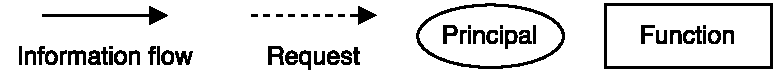
\includegraphics[scale=0.8]{figures/dlm_legend}
\end{figure}
In the graphs we have two abstractions that are not apparent when looking at the source code.
The main function has been left out, and the \emph{request} flows represent calls to the program through some means (e.g. a call from another program or through a web-request).
In the code source, the logic in the main function will also not represent an actual implementation, as we have abstracted away from how the program will actually be called.

\subsection{Smart meter bill calculation}
Related to the protection of smart meter data, we have created a simple example (see \cref{example:code:calculate_bill} and \cref{example:graph:calculate_bill}) which uses data from both consumer and electrical company in order to calculate a bill.
Here we make use of 4 declared auxiliary functions: \dlmc{get_latest_usage}, \dlmc{get_latest_prices}, \dlmc{send_to_consumer}, and \dlmc{send_to_electrical_company}.
The actual implementation of these is not important, they are only seen to represent ways of either obtaining data from outside the program, or sending data to outside of the program.
\mikkelin{Describe how the use of two nested while loops is enough to make it hard for the programmar to determine what the actual information flow is.}
\mikkelin{Include itemize with forward reference for labeled version of the example and time-construct thingies.}

\lstinputlisting[float, style=dlmc, numbers=left, caption={Smart meter bill calculation example}, label=example:code:calculate_bill]{dlm_examples/report/calculate_bill.ncif}
\begin{figure}
  \centering
  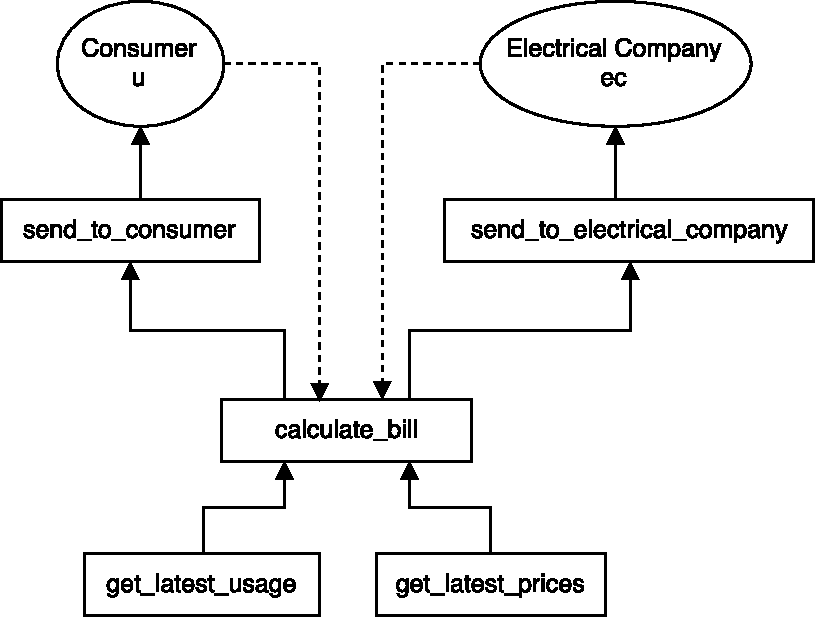
\includegraphics[scale=0.8]{figures/dlm_calculate_bill}
  \caption{Information flow graph for \dlmc{calculate_bill}}
  \label{example:graph:calculate_bill}
\end{figure}

\subsection{Password checker}\label{example:sec:check_password}
A more general example is a password checker (see \cref{example:code:check_password} and \cref{example:graph:check_password}), which takes a username and password combination and checks it against the user database, giving a response to the user whether it was correct or not.
\mikkel{Why is the password checker more general? - Password checking is found in many devices.}
Here we have 3 auxiliary functions: \dlmc{get_login}, \dlmc{get_users}, and \dlmc{send_response} -- they represent the two inputs needed, as well as the response to be given.
\mikkelin{Include itemize with forward reference for labeled version of the example and time-construct thingies.}

\lstinputlisting[float, style=dlmc, numbers=left, caption={Password checker example}, label=example:code:check_password]{dlm_examples/report/check_password.ncif}
\begin{figure}
  \centering
  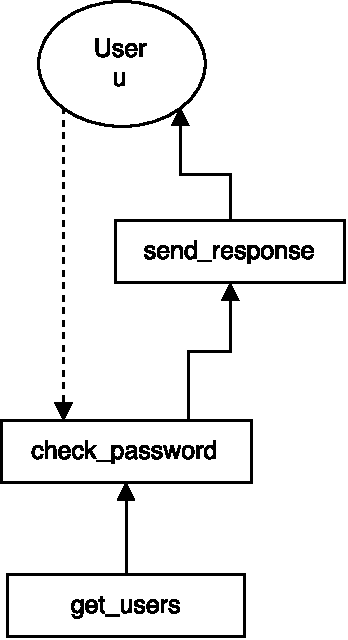
\includegraphics[scale=0.8]{figures/dlm_check_password}
  \caption{Information flow graph for \dlmc{check_password}}
  \label{example:graph:check_password}
\end{figure}


% !TEX root = ../master.tex

\newcommand{\labelof}[1]{\underline{#1}}
\newcommand{\dlmc}[1]{\lstinline[style=dlmc]{#1}}
\newcommand{\dlmactsfor}{\dlmc{if\_acts\_for}}
\newcommand{\dlmdeclassify}{\dlmc{declassify}}
\newcommand{\dlmpc}{$\underline{pc}$}
\newcommand{\mathcomment}[1]{\color{green!50!black}{#1}}

\section{The Decentralized Label Model}
The Decentralized Label Model \cite{myers1997, myers1998, myers2000} is a model for ensuring information flow control in a system.
This is done by annotating source code with security policies, in the form of labels attached to data-holding constructs.
This section will present the necessary information needed to understand the implementation of \thetool.
The descriptions and definitions in this section are based on \cite{myers1997, myers1998, myers2000}.
Throughout the examples, we will use the same grammar as that used by \thetool. \mikkel{Remember to write something about the grammar/parser...}

\subsection{Labels and Policies}
Throughout a program, values are declared, initialized, and assigned to variables and other value-holders.
Value-holders are collectively known as \emph{slots}, which cover constructs such as variables, structs, and other storage locations.
In order to ensure that a certain assignment is legal, such that no information is unintentionally leaked, we assign \emph{labels} to slots so that their ``security'' can be compared.
This way we can ensure that an assignment is only legal in the cases where higher-security values aren't assigned to lower-security slots.
The same concept applies to more complex language constructs, such as functions (and their return values).

Each slot is associated with a label, that describes how the data in the slot can be handled.
We denote the label of slot $s$ as $\underline{s}$.
Referring to labels in this fashion serves the same purpose as letters in algebra; it allows for handling labels without knowledge about their actual value.
This proves useful as it allows for label inference and label polymorphism (see \cref{dlm:implicit_labels} and ??). \mikkel{Insert reference when written.}\mikael{Are we going to write about label polymorphism?}

For a given label it is possible to define both read (\emph{privacy}) and write (\emph{integrity}) policies.
The first represents information flow out of a system and the latter information flow into a system.
In this report only read policies will be considered.
Due to the relation between the two types of policies, we note that write policies can be ensured in a fashion similar to read policies.
Because of this we choose to simplify the scope of the report such that it only discusses read policies.

\subsubsection{Principals}
In the following, we employ the concept of \emph{principals}.
A principal (or \emph{subject}, \emph{agent}) is an entity in a system that represents some interest.
In short, principals represent real-world users or the authority under which a program/system runs.
Principals can exists in a \emph{principal hierarchy}, that describe more complex principal relationships, such as groups or roles.
\mikkel{Reminder about principal hierarchies}
In the following we make use of the special set of principals; $*$.
This set represents all principals in a system.

\subsubsection{Labels}
A label can be described as a set of policies, where a policy consists of an owner principal $o$ and a set of reader principals $r_1, r_2, \dots, r_n$.
Formally we provide the following, equivalent definition:
\begin{definition}{Labels}
A label $L$ is a set of owners $owners(L)$, and a function $readers(L, o)$ that retrieves the set of reader principals that $o$ allows to read.
Note that given this definition we have that $$o \notin owners(L) \Rightarrow readers(L, o) = *$$
\end{definition}

Owners are allowed to change their own policies within a label.
We describe how this is done in \cref{dlm:auth_and_declass}.
If an owner is not part of its own policies reader set, that owner is not allowed to read from the slot associated with the label.
He is however still allowed to change his policy.

\subsubsection{The effective reader set}
To ensure that the policies of all owners in a label are enforced, only readers that the all ``agree'' on can read from the slot associated with the label.
This is known as the \emph{effective reader set}, which is the intersection of \emph{all} reader sets of a label:
\begin{definition}{The effective reader set}
  $$readers(L) = \bigcap_{o \in *} readers(L, o)$$
\end{definition}

\begin{example}{A label with two policies}\label{dlm:ex:simple_label}
  Below is an example of a label with two policies using the notation from above;
  $$L_1 = \{o1 \rightarrow r1, r2; o2 \rightarrow r2, r3\}$$

  The owner set of the label is $owners(L_1) = \{o1, o2\}$, and its reader sets are $readers(L_1, o1) = \{r1, r2\}, readers(L_1, o2) = \{r2, r3\}$.
  By intersecting the reader sets of the label we get the effective reader set.
  In practice we can disregard the reader set of labels that are not owners.
  Thus the effective reader set is
  $$readers(L_1) = \{r1,r2\} \cap \{r2, r3\} = \{r2\}$$
\end{example}

\subsubsection{Label comparison}
As mentioned above, labels provide restrictions on which principals can read from the slots that the labels ``protect''.
In order to check that security policies are enforced throughout a program, we need to be able to compare how restrictive labels are.
To do this we introduce the ``at most as restrictive as''-relation ($\sqsubseteq$) from \cite{myers1997}.


\begin{definition}{Label Comparison Rule}
  \begin{align}
    \text{For } & L_1 \sqsubseteq L_2 \text{ we have that} \nonumber \\
    & owners(L_1) \subseteq owners(L_2) \text{ and} \nonumber \\
    & \forall o \in owners(L_1) . readers(L_1, o) \supseteq readers(L_2, o) \nonumber
  \end{align}
\end{definition}

\subsubsection{Label join}
In order to compare composite labels, such as those for arithmetical expressions, we need to be able to create and use a ``joined label''.
This is also needed when we consider implicit flows via scope blocks, as will be described in \cref{dlm:implicit_flows}.
The result of a label join is the least restrictive label that maintains all flow restrictions.
Since each label is a set of policies, the definition of label join ($\sqcup$) is simply:

\begin{definition}{Label Join Rule}
  \[
    L_1 \sqcup L_2 = L_1 \cup L_2
  \]
\end{definition}

\begin{example}{Joining of two labels}
  If we have the two initializations:
  \begin{lstlisting}[style=dlmc]
int {{a->z,y}} val1 = 4;
int {{b->x,w}} val2 = 8;
  \end{lstlisting}
  The joined label of the expression\\
  \begin{lstlisting}[style=dlmc]
val1 + val2
  \end{lstlisting}
  is
  \begin{lstlisting}[style=dlmc]
{{a->z,y; b->x,w}}
  \end{lstlisting}
  Since we have the implicit least restrictive policies for $b$ and $a$ in \dlmc{val1} and \dlmc{val2} respectively.
\end{example}

\subsubsection{Security class lattice}
By having this relationship between labels, we can see the set of all our labels as a partially-ordered set: a \emph{lattice}.
This means that we have a hierarchy, in which the shared parent of every two individual elements is the result of a join ($\sqcup$) of the two labels, as well as a shared child: the result of a meet ($\sqcap$) of the same two labels.
Additionally, to represent the least restrictive label of any security class lattice we have a bottom element, denoted $\bot$.
Dual to the bottom element, we also have the most restrictive label: the top element, denoted $\top$.

\subsection{Implicit flows}\label{dlm:implicit_flows}
When assigning a value to a slot, possibly from another slot, it is an explicit flow.
In addition to explicit flows, it is also possible to have implicit flows throughout a program, due to conditional control structures (such as loops).
For whatever assignments we would do inside a block (or within a deeper block hierarchy) we need to take the predicates of these blocks into consideration.
This is done by adding the concept of \emph{program counter labels}, denoted \dlmpc.
For each scope we will have an implicit \dlmpc, depending on the surrounding predicates' labels.

\begin{example}{Implicit leak}\label{dlm:ex:implicit_leak}
  Consider the following program (each line commented with the current \dlmpc):
  \begin{lstlisting}[style=dlmc]
int {{a->z,y}} val = 0;   // $\mathcomment{\bot}$
int {{a->y}} cond = 1;    // $\mathcomment{\bot}$
if (cond) {
  val++;                  // $\mathcomment{\bot \sqcup \{a \rightarrow y\}}$
}
return val;               // $\mathcomment{\bot}$
  \end{lstlisting}
  In this example we would have an implicit leak of \dlmc{cond}, by way of \dlmc{val}.
  This is due to the assignment of \dlmc{val} inside of the \dlmc{if}-statement, as \dlmpc~ is increased to the join of the outer scope ($\bot$) and the label of the scope's predicate (\labelof{\dlmc{cond}}).
  For this program to pass \thetool, we would have to add a more strict policy to \dlmc{val}, so that it could match the policy of \dlmc{cond}.
\end{example}

\subsection{Authority and declassification}\label{dlm:auth_and_declass}
In order to avoid mishaps by setting certain policies too lax, so that certain flows are permitted, we can temporarily set some policies to be more strict, and then only relax (\emph{declassify}) them when we really need to.
In order to do this, we need the concept of \emph{authority}.
At any point during running a program, it will have a \emph{true authority}, which is the maximal authority by which the program can carry out operations.
Whenever we call a function, we can do this with a certain authority, corresponding to running that method with the authority of a specific principal.
However, in order to take advantage of this given authority, we need to explicitly claim it.
This is done by using the \dlmactsfor\dlmc{(a, b) \{ stmts \}} statement, where $a$ is the principal (typically the function itself) trying to obtain the authority of $b$.
Only after calling this function will we obtain the \emph{effective authority} to act for $b$, enabling us to carry out the statements within the \dlmactsfor~ block that would normally only be permissible for $b$ itself.

If the check passed, then we will inside the \dlmactsfor~ block now have the ability to carry out operations that normally would be permissible only to $b$ itself.
Most importantly, we can do declassification -- deliberately and explicitly relaxing the security policies in which $b$ is owner.
This is done by calling the \dlmdeclassify\dlmc{(v, l)} function, with a slot $v$ and a new label $l$ as inputs, returning the value $v$ relabeled to $l$.
The relabeling by declassification rule (the inference rule) is defined as follows:

\begin{definition}{Relabeling by declassification}
  Let $P$ denote the set of principals in the current authority, then
  \[
  \frac
  {
    \splitfrac
    {
      L_A = \mathlarger\sqcupl_{p \in P} \{p \rightarrow \}
    }
    {
      L_1 \sqsubseteq L_2 \sqcup L_A
    }
  }
  {
    L_1 \text{ may be declassified to } L_2
  }
  \]
\end{definition}

The combination of these two concepts, \dlmactsfor~ and \dlmdeclassify, is especially useful when we have sensitive inputs to a method and want to carry out our calculations without the fear of neither explicit or implicit leakage.
This way we can keep our strict policies throughout the calculations of the method and only relax the label once we want to return the result.

\begin{example}{Temporarily restricting a label}
  Building on \cref{dlm:ex:implicit_leak}, we can set the label for \dlmc{val} to match that of \dlmc{cond}, and then only relax that label when we need to return \dlmc{val}, ensuring that we have the ability to do so:
  \begin{lstlisting}[style=dlmc]
int {{a->y}} val = 0;
int {{a->y}} cond = 1;
if (cond) {
  val++;
}
if_acts_for(this, a) {
  return declassify(x, {{a->y,z}});
}
return -1;
  \end{lstlisting}
  While we still leak some information about \dlmc{cond}, we now do it explicitly.
\end{example}

\subsection{Label-checking and inference}


\chapter{Decentralized Label Model in C}\label{ctif}
% !TEX root = ../../master.tex

In this chapter we will present the \thelanglong{} language, hereafter referred to simply as \thelang.
However, this chapter will only show how to apply ordinary labels, as those presented in the previous chapter.
The following chapter will go into the details of time policies.\mikael{Bedre forklarende meta.}

\thelang{} is based upon C99 and will extend the syntax of C with the concept of labels, as discussed in the previous chapter.
This fact gives us two nice properties:
\begin{enumerate}
  \item A C99 program\footnote{Limited under the scope presented in \cref{ctif:scope}.} is compilable with the \thelang{} compiler.
  \item An unlabeled \thelang{} program can be checked by a C99 compiler.
\end{enumerate}
The first property allow for incrementally adding labels to old source code.
This becomes even more palpable when also having the ability of using the \thelang{} compiler to infer labels.
The second property frees the \thelang{} compiler from handling many of the same things that instead can be handled by already existing C99 compilers.
\mikael{Fordele ved ikke at skrive hel C compiler.}

The rest of this chapter will be organized as follows.
Firstly, we will present the scope under which we have limited our implementation.
Then we will informally present \thelang.
Lastly we will present the specifics of extracting constraints, to be used for inferring labels, as was described in \Cref{dlm:constraints,dlm:inferring_labels}.

% !TEX root = ../../master.tex

\section{Scope}\label{ctif:scope}
We have tried to include as many C constructs as possible, in order to properly ascertain the usefulness of \thelang.
However, certain aspects of C have been either simplified or completely left out.

In the following is a crude list with what is currently supported in \thelang.
Following the list will be some elaborations where necessary.
\begin{itemize}
  \item Variables
  \item Simple types (int, bool, char, string)
  \item Structs
  \item Pointers
  \item Function prototypes, declarations, and calls
  \item Boolean and arithmetic operators
  \item \emph{if}- and \emph{while} control statements
  \item External libraries
\end{itemize}

\myparagraph{Structs and arrays}
It is possible to define structs, so that the defined type can be used similarly to any other type.
Both structs and arrays can be declared, arrays by using pointer-notation.
However, it is not possible to initialize neither struct or array.
We still have index and element expressions, with a simple implementation, which only takes into account the label of the struct/array variables.

We have chosen to leave initilization for structs and arrays out for now, as we found no proper solution for handling policies for individual fields and elements.
In \cite{myers1997} labels can be applied to structs by labeling the variable.
Additionally, fields can be labeled, resulting in a special rule for the evaluation of accessing struct fields, which is the label join of the struct label and the accessed field's label.
We, however, find it somewhat illogical to label a type, since different usage of a certain type may call for different labeling.

\myparagraph{Pointers}
Similar to both \cite{muller2015cif} and \cite{maciazek2016cbif} we allow for pointer declarations and for the two pointer operations dereference and address-of, but disallow pointer arithmetics.
Pointer arithmetics is deemed too big of a subject to handle within the scope of this report, and without proper handling it is potentially highly error-prone.\footnote{\url{https://www.securecoding.cert.org/confluence/display/c/EXP08-C.+Ensure+pointer+arithmetic+is+used+correctly}}

\myparagraph{Boolean and arithmetic operators}
The following boolean and arithmetic operators are allowed:
\[ \tk +, \tk - \text{(unary and binary)}, \tk *, \tk /, \tk{\&\&}, \tk{||}, \tk{!}, \tk * , \tk \& \]

Operator precedence has no say for our compiler, as we are only interested in what operands are used in expressions.
The actual operator precedence checks are only used for, and therefore handled by, the C compiler.

\section{Informal Description}
\thelang{} extends the C language with the ability to declare labels for values and functions.
Labels are declared between the type and the identifier of a variable, or between the return type and identifier of a function.
The syntax for labels consists of 5 components:
\begin{itemize}
  \item delimiters \dlmc{\{\{ \}\}}
  \item join operator \dlmc{;}
  \item identifiers -- e.g. \dlmc{owner}, \dlmc{reader}, or \dlmc{variable}
  \item policy operator \dlmc{->} -- e.g. \dlmc{\{\{owner->reader1, reader2\}\}}
  \item special values \dlmc{_} (underscore, for bottom label) and \dlmc{^} (caret, for top label)
\end{itemize}

Besides the actual labels we also have the 3 related constructs, which were presented in \cref{dlm:auth_and_declass,dlm:channels}:
\begin{itemize}
  \item output channel \dlmc{p1, p2 <- foo();}
  \item if acts for \dlmc{-->? p1, p2 \{ /* statements */ \}}
  \item declassify \dlmc{<|v, l|>}
\end{itemize}

The following subsections will describe how labels are used in \thelang.
The descriptions will follow the password checker example from \cref{example:sec:check_password}.
The fully labeled source can be seen in \cref{example:code:check_password-explicit}.

\lstinputlisting[float, style=dlmc, numbers=left, caption={Labelled password checker example}, label=example:code:check_password-explicit]{dlm_examples/report/check_password-explicit.ncif}

\subsection{Function declarations}
The first thing we would want to label in a program is what can be seen as the bigger components; the functions that either obtain data from outside or send data to outside the program -- our channels.
In \thelang{} we have no distinction between input channels and any other function which has a return value.
However, output channels are distinguishable by having the \dlmc{<-} construct, preceded by one or more principals (readers).
Output channel declarations are initially checked as with any other function.

For \dlmc{check_password} we have the 3 auxiliary functions, as well as the \dlmc{check_password} function itself, which we would label as so:\\
\begin{minipage}{\linewidth}
\lstinputlisting[style=dlmc, numbers=left, linerange={11-15}, firstnumber=11]{dlm_examples/report/check_password-explicit.ncif}
\end{minipage}

Here we have two principals: user (u) and password checker (pc).\footnote{We make use of the \dlmc{principal} declaration in the full example to simulate the actual obtaining of system principals.}
The user provides some login information, to which he is the owner.
The password checker is a trusted principal which has access to the user database.
The final output is sent to an output channel which is readable only be the user.

\dlmc{check_password} returns the comparison result, which is owned by and readable by the user only.
Here we also need to add labels to the parameters, otherwise we would not be able to statically check the function, as the actual labels for the parameters could differ between different calls to the function, but by supplying the labels we know that the policies will have to hold for all usage.
When supplied with a label, parameters are treated as any other variable when evaluating a function declaration.
However, if no label is supplied for a parameter, that parameter is recognized as labeled with a constant label.

\subsection{Variable declarations}
The labeling of variable declarations is done mainly to oblige the return values of functions and input, given by either parameters or auxiliary function calls.
This is also why most of these labels are easier to infer, and can therefore often be left out, as we shall see later in this section.

For \dlmc{check_password} we have the following labeling of variables:\\
\begin{minipage}{\linewidth}
\lstinputlisting[style=dlmc, numbers=left, linerange={16-19}, firstnumber=16]{dlm_examples/report/check_password-explicit.ncif}
\end{minipage}

The labeling applied here is done so that it obliges the different inputs to the method.
The most noteworthy here is the labeling of \dlmc{match}, as it through its assignment within both the \dlmc{while} and \dlmc{if} blocks will implicitly obtain knowledge of all other labeled values.
It is therefore labeled with the join of all those labels: \dlmc{\{\{u->u;pc->\}\}} so that it is at most as strict as all.

\subsection{If-acts-for and declassification}\label{ctif:informal:ifactsfor_declassify}
Going into \dlmc{check_password} we have data that is privy to the user as well as data that is not.
So before we can return the result to the user, we need to explicitly declare that in this particular case it is an intentional leak of the password checker's data (the user db).

This is done with the declassification delimiter \dlmc{<| |>} which takes two arguments, an expression to be declassified and the new label.
For \dlmc{check_password} we need to declassify and return \dlmc{match}:\\
\begin{minipage}{\linewidth}
\lstinputlisting[style=dlmc, numbers=left, linerange={28-30}, firstnumber=28]{dlm_examples/report/check_password-explicit.ncif}
\end{minipage}

As can be seen we also need to obtain the proper authority before such a declassification is possible.
This is done by using the \emph{if-acts-for} statement, identified by the \dlmc{-->?} syntax, which is preceded by type of authority and followed by principals to acquire authority for.
During compile-time checking we do not differ between the special keywords \dlmc{this} and \dlmc{caller}.
After obtaining the proper effective authority, we need to clear the return value's label of the policy of \dlmc{pc}, as explained in the beginning of this subsection.

It is possible to leave out the explicit label of the declassification, as we will see in the following subsection.

\subsection{Inference}
As we have argued repeatedly throughout this report, having to declare labels for every value or function can be time-consuming and can cause a clutter in a program.
Therefore we can rely on inference so that many labels can be omitted.
In \cite{myers1997} it is only described what leaving out labels for variables and parameters mean, and not functions.
Therefore we have reasoned about the implications of leaving out the function label and come up with a reasonable solution, so that we can leave out those labels and still expect proper results.

As we have seen, explicit labels can be applied to the three types of declarations: function, parameter, and variable, as well as in the declassification expression.
Here we will explain what it means to leave out any of those labels in a program.
An overview of the different rules that apply are given here:
\begin{table}[H]
  \begin{tabularx}{\textwidth}{|l|X|}
    \hline
    \textbf{Construct} & \textbf{Default label} \\ \hline \hline
    Variable & Variable label \\ \hline
    Declassification & Variable label \\ \hline
    Function & The join of all parameter labels \\ \hline
    Parameter & Constant label \\ \hline
  \end{tabularx}
  \caption{Default labels for unlabeled constructs}
  \label{informal:table:default_labels}
\end{table}

As described in \cref{dlm:inf:types}, we have the concepts of \emph{variable labels} and \emph{constant labels}.
Variable labels are the main enablers of the inference algorithm, as it allows for implicitly labeling certain values that in themselves do not need a label, but are instead related to other values that do.
Constant labels, in a similar fashion, allow for the abstraction of only applying labels where it is critical, allowing for some implicity when defining the security of functions.
We have updated the password checker example (see \cref{example:code:check_password-implicit}), removing all explicitly declared labels that instead can be inferred.
Similarly, the calculate bill example has been labeled as well (see \cref{example:code:calculate_bill-implicit}).

\lstinputlisting[float, style=dlmc, numbers=left, caption={Labeled password checker example -- with default labels}, label=example:code:check_password-implicit]{dlm_examples/report/check_password-implicit.ncif}

\lstinputlisting[float, style=dlmc, numbers=left, caption={Labeled smart meter bill calculation example -- with default labels}, label=example:code:calculate_bill-implicit]{dlm_examples/report/calculate_bill-implicit.ncif}

\myparagraph{Variable}
As explained above, by removing the explicitly declared label for a variable, we instead rely on the inference algorithm to satisfy any constraints.
Since we have explicitly declared the labels for all our channels and \dlmc{check_password}, we do not need to explicitly label all our variables as well.
This results us in being able to leave out all label declarations for variables.

\myparagraph{Declassification}
Similar to variables, we can leave out the explicitly declared label for the declassification expression.
This creates a variable label for that expression, so that we can rely on inference in a similar fashion as with any other value labeled with a variable label.

\myparagraph{Functions and parameters}
If no explicitly declared label is found for a function declaration, the label defaults to a join of all parameter labels ($\bot$ if the function has no parameters).
This is based on an assumption about the minimum security needed for a function, in that whatever a function returns can be related to at most whatever arguments are given.
This is useful for declaring auxiliary functions, without having to explicitly declare the security implications of such a function.

For our password checker we could declare an auxiliary function \dlmc{strcicmp}, for doing a case-insensitive check of usernames, with the following prototype:\\
\begin{minipage}{\linewidth}
  \centering
  \dlmc{bool strcicmp(char *a, char *b);}
\end{minipage}
\dlmc{stricmp} would then have the label \dlmc{\{\{a;b\}}}, per our default label for function declarations, and any evaluation of calls to \dlmc{stricmp} would result in a label which is the join of all its arguments.
This is the default behaviour of library functions, which can be overridden by declaring a labeled prototype with the corresponding library function signature.

Extending on the concept of referencing parameter labels in function return labels, we can choose which parameters to reference.
If we take the function \dlmc{stricmp} and want to extend it with a maximum amount of characters to compare before failing, we could have that its signature was:\\
\begin{minipage}{\linewidth}
  \centering
  \dlmc{bool \{\{a;b\}\} stricmp(char *a, char *b, int max_length);}
\end{minipage}
Similar to the previous example, we have that any calls to \dlmc{stricmp} will be evaluated to the join of its arguments, but this time only the arguments \dlmc{a} and \dlmc{b}, thus any security applied to \dlmc{max_length} will not affect the label of the return value.

% !TEX root = ../../master.tex

\section{Constraint Extraction}\label{extraction}
In this section we will give a formal definition of how constraints are extracted from a \thelang~ program.
This formal definition will be based on denotational semantics, and will therefore utilize the concepts thereof.
We will define our syntactic and semantic setup, which will serve as a base for the rules for how constraints are extracted from a \thelang~ program.
Following the setup, we will present the semantic equations, which describe how constraints are extracted from the individual program constructs.

\subsection{Syntax}
Below follows an abstract syntax that describes the structure of our grammar.
The grammar is made to represent the C programming language in both structure and actual syntax.
The latter is not directly apparent here, as some syntactical details have been removed to achieve a higher level of abstraction.

\begin{table}[p]
  \begin{align*}
    R       & \in \iProg \text{ -- Programs}\\
    D       & \in \iDec \text{ -- Declarations}\\
    D_F     & \in \iDecf \text{ -- Function declarations}\\
    f       & \in \iFun \text{ -- Functions}\\
    D_V     & \in \iDecv \text{ -- Variable declarations}\\
    x       & \in \iVar \text{ -- Variables}\\
    p       & \in \iPrin \text{ -- Principals}\\
    S       & \in \iStm \text{ -- Statements}\\
    E       & \in \iExp \text{ -- Expressions}\\
    L       & \in \iLbl \text{ -- Label declaration}\\
    P       & \in \iPol \text{ -- Policy declaration}\\
    op_b    & \in \{ \tk + ,  \tk - ,  \tk * ,  \tk / ,  \tk \% ,  \tk{||} ,  \tk{\&\&} ,  \tk < ,  \tk > ,  \tk{==} ,  \tk{<=} ,  \tk{>=} \} \\
    op_u    & \in \{ \tk ! ,  \tk - , \tk * , \tk \& \} \\
    k       & \in \{ \tk{true}, \tk{false} \} \cup \mathbf{Num} \cup \mathbf{Chr} \cup \mathbf{Str} \text{ -- Boolean, integer, char, and string literals} \\
    t       & \in \mathbf{Types} \text{ -- C types (including defined structs)}
  \end{align*}
  \begin{align*}
    R         & ::= D \\
    D         & ::= D_F \gp D_V \gp D_1 \; D_2 \\
    D_F       & ::= p_1 \tk , p_2 \tk , \dots \tk , p_k \tk{<-} \; t_f \; l_f \; f \tk ( t_1 \; l_1 \; x_1 \tk , t_2 \; l_2 \; x_2 \tk , \dots \tk , t_n \; l_n \; x_n \tk ) S \\
    D_V       & ::= t \; l \; \tk * x \tk = E \gp t \; l \; \tk * x \\
    S         & ::= E \gp S_1 \; S_2 \gp \varepsilon \\
              & \gp D_V \\
              & \gp \tk{while} \tk ( E \tk ) S \gp \tk{if} \tk ( E \tk ) S \gp \tk{if} \tk ( E \tk ) S_1 \tk{else} S_2 \\
              & \gp x \tk = E \\
              & \gp \tk{return} E \gp \tk{return} \\
              & \gp \tk{this} \tk{-{}->?} p_1 \tk , p_2 \tk , \dots \tk , p_k \; S \gp \tk{caller} \tk{-{}->?} p_1 \tk , p_2 \tk , \dots \tk , p_k \; S \\
    E         & ::= x \gp k \gp E_1 \; op_b \; E_2 \gp op_u \; E \gp \tk ( E \tk ) \gp E \texttt{.} x_f \gp E \texttt{->} x_f \gp x \texttt{[} E \texttt{]} \\
              & \gp \tk{<|} E \tk , l \tk{|>} \gp \tk{<|} E \tk{|>} \\
              & \gp f \tk{<{}<{}<} p_1 \tk , p_2 \tk , \dots \tk , p_k \tk{>{}>{}>} \tk ( E_1 \tk , E_2 \tk , \dots \tk , E_n \tk ) \\
    L         & ::= \tk{\{\{} P \tk{\}\}} \gp \varepsilon \\
    P         & ::= x \gp p_0 \tk{->} p_1 \tk , p_2 \tk , \dots \tk , p_k \gp P_1 \tk ; P_2 \gp \tk \_ \gp \tk{\^{}}
  \end{align*}
  \caption{Syntactic domains and abstract production rules}
  \label{ctif:rules}
\end{table}

\Cref{ctif:rules} primarily serve as a reference-point for the following sections.
We will however briefly discuss a few details that might be of special interest:

\paragraph{Simplified arithmetics}
As the semantics, described in this section, only concerns how data \textit{flows} and not its value on execution we can simplify the possible binary and unary operations into two rules.
Doing so provides for a less cluttered syntax and a clearer focus on the label semantics that are expressed.

\paragraph{Pointer declaration}
The \tk{*} used in variable declarations, to indicate a pointer declaration, is optional.
Whether a variable is a pointer or not has no meaning for the evaluation of labels, so the handling of pointer type checking is completely left to the C compiler.
Therefore it will not be apparent in the syntax in the rules for variable declaration.

\paragraph{Struct fields}
We make use of the special identifier $x_f$ for struct fields access.
It has no meaning in evaluating the program, as will be apparent in the rules for the struct field expression.
The actual checking of struct fields and the matching struct definition is handled by the C compiler.

\paragraph{Empty labels}
No value (represented by $\varepsilon$) can be provided for any label declaration.
When omitting a label the semantic rules specify a \textit{default} value for the label.
This is initial step of label inference and allows unlabeled C to be recognized and evaluated using these rules.

\subsection{Semantic setup}
This section will describe the semantic constituents which are used to translate a syntactical \thelang{} program into the semantical world.
These constituents are based on the concepts: \emph{semantic domains}, \emph{semantic functions}, and \emph{semantic equations} from \cite[Chapter 9]{slonneger1995formal}.
The semantic domains and semantic functions will be described in the next two subsections.
For readability purposes, the semantic equations will be spread out over the following subsections.

\subsubsection{Semantic domains}
The semantic domains of \thelang{} are primarily used to maintain state, and to give the final result of the constraint extraction: namely the constraints themselves as well as the different label types which are used to form the constraints.
Note that we have no need for any numerals or type enumerations, since we are only interested in checking labels and forming constraints.

The following list is an overview of these semantic domains (Here $\mathcal P$ denotes the power set):
\begin{align*}
\iLV    & = v(\iVar) \cup c(\iVar) \cup p(\mathbb{L}) \cup j(\iLV \times \iLV) \\
\iCstr  & = \mathcal P (\iLV \times \iLV) \\
\iEnvF  & = \iFun \cup \{ \ifb \} \rightharpoonup \iLV \times \mathcal P (\iLV \times \iVar) \times \mathcal P(\mathbb{P}) \\
\iEnvL  & = \iVar \cup \{ \ia, \ib \} \rightharpoonup \iLV
\end{align*}

$\mathbb L$ denotes the set of all labels.

$\mathbb P$ the set of all principals.
Principals are expected to be extracted from some system information and not defined in the program code itself.
Instead we make us of a function $principal$, which is used to represent the lookup of principal names in some system:
\[ principal = \iPrin \rightarrow \mathbb P \]
We will also make use of the special set $P^*$, where $P^* \subseteq \mathbb{P}$, representing all principals of the system.

$\iLV$ is a set of \emph{label values}, not to be confused with actual labels.
In order to differ between the different types of labels (as described in \cref{dlm:inf:types}), we utilize concept of \emph{tagged values}.
Each element in $\iLV$ is then on the form $t(v)$, where $t$ is the type of label and $v$ is the value, which then differs depending on the type of label.

To further increase readability when using \emph{join labels}, we will introduce another notation using quotes to signify that the value is the constituents and not the evaluated expression.
Then we have that:
\[ \literal{\ilv_1 \sqcup \ilv_2} \equiv j(\ilv_1, \ilv_2) \]

$\iCstr$ is a set of constraint tuples, where any $(\ilv_1, \ilv_2) \in \iCstr$ can be seen as representing a constraint: $" \; LV_1 \sqsubseteq LV_2 \; "$.
Similar to the join label above, we will have the latter notation in quotes having the same meaning as the aforementioned tuple, such that:
\[ \literal{\ilv_1 \sqsubseteq \ilv_2} \equiv (\ilv_1, \ilv_2) \]

When we have both $\sqcup$ and $\sqsubseteq$ in a ``quoted expression'', the precedence is $\sqcup$ before $\sqsubseteq$.

$\iEnvL$ is the label environment, which maps variable identifiers, and the two special identifiers $\ia$ (authority) and $\ib$ (block), to label values.
The special values are propagated throughout a program, as they will change as the scope changes.

$\iEnvF$ is the function environment, which maps function identifiers, and the special identifier $\ifb$ (function block), to a tuple containing the label value of the function along with all its arguments and output readers.
Function identifiers are looked up when evaluating function calls.
The function block identifier is used for return statements so that the ``surrounding'' function label can be looked up.

\subsubsection{Semantic functions}
The semantic functions describe how the syntactic domains (see \cref{ctif:rules}) will be transformed into the semantic domains described above.
We have a function for each domain from which we need to extract constraints, or from which we need to derive the labels used in forming constraints.
The formal definitions of the semantic functions can be seen in \cref{cstr:semantic_functions}.

\begin{table}[H]
\begin{align*}
  \iR & : \iProg \rightarrow \iCstr \\
  \iD & : \iDec \rightarrow (\iEnvL \times \iEnvF \rightarrow \iCstr \times \iEnvL \times \iEnvF) \\
  \iF & : \iDecf \rightarrow (\iEnvL \times \iEnvF \rightarrow \iCstr \times \iEnvF) \\
  \iV & : \iDecv \rightarrow (\iEnvL \times \iEnvF \rightarrow \iCstr \times \iEnvL) \\
  \iS & : \iStm \rightarrow (\iEnvL \times \iEnvF \rightarrow \iCstr \times \iEnvL) \\
  \iE & : \iExp \rightarrow (\iEnvL \times \iEnvF \rightarrow \iCstr \times \iLV) \\
  \iL & : (\iLbl \cup \iPol) \rightarrow (\iEnvL \rightarrow \iLV \cup \{ \varepsilon \})
\end{align*}
\caption{Semantic functions}
\label{cstr:semantic_functions}
\end{table}

The ``entry point'' of a \thelang{} program is simply one or more declarations, and the result of evaluating such a program is always a set of constraints.
The transformation of declarations will result in a set of constraints, as well as a changed environment: function for function declarations and label for variable declarations.
Statements are where most constraints will originate from, as this is where we have both variable declarations and assignments.
Expressions will also generate constraints, due to the ability to use declassifications.
Due to the simplicity of the label syntactic domain, its rules has been merged with those of policy.
Unlike the previous semantic functions, labels and policies are only evaluated to a label value in order to use them in the forming of constraints.

\subsection{Program and declarations}
The rules for program and declarations are simple, as their main purpose is providing an entry point, as well as the ability to have variable and function declarations appear in the global scope, and in arbitrary order.
$empty\ienvF$ and $empty\ienvL$ are the initial, empty, environments.

\begin{table}[H]
\begin{semanticequations}
% Program
\csemeq{\iR}{D}{}{\icstr}{
  \seWhere{\semeq{\iD}{D}{empty\ienvL \; empty\ienvF}{(\icstr, \ienvL, \ienvF)}}
} \seSpace
% Function Declaration
\csemeq{\iD}{D_F}{\ienvL \; \ienvF}{(\icstr, \ienvL, \ienvF_2)}{
  \seWhere{\semeq{\iF}{D_F}{\ienvL \; \ienvF}{(\icstr, \ienvF_2)}}
} \seSpace
% Variable Declaration
\csemeq{\iD}{D_V}{\ienvL \; \ienvF}{(\icstr, \ienvL_2, \ienvF)}{
  \seWhere{\semeq{\iV}{D_V}{\ienvL \; \ienvF}{(\icstr, \ienvL_2)}}
} \seSpace
% Composite Declaration
\csemeq{\iD}{D_1 \; D_2}{\ienvL \; \ienvF}{(\icstr \cup \icstr_2, \ienvL_3, \ienvF_3)}{
  \seWhere{\semeq{\iD}{D_2}{\ienvL_2 \; \ienvF_2}{(\icstr_2, \ienvL_3, \ienvF_3)}} \\
  \seAnd{\semeq{\iD}{D_1}{\ienvL \; \ienvF}{(\icstr, \ienvL_2, \ienvF_2)}}
}
\end{semanticequations}
\caption{Semantic equations for program and declarations}
\label{cstr:program_declarations}
\end{table}

\subsection{Label and policy}\mikael{We may need to differ between policy labels and label constituents/composite labels)?}
The rules for labels and policies consist of a simple transformation of the syntactical labels into their semantic equivalents.
Worth noting here is that there is no ``empty'' label value for undeclared labels.
As the label value for an undeclared label depends on its context, $\varepsilon$ is simply passed through on evaluation.

\begin{table}[H]
\begin{semanticequations}
% Empty
&\semeq{\iL}{\varepsilon}{\ienvL}{\varepsilon} \seSpace
% Policy
&\semeq{\iL}{\tk{\{\{} pol \tk{\}\}}}{\ienvL}{\iL [\![pol]\!] \; \ienvL} \seSpace % gives error when using semeq commands
% Composite Policy
\csemeq{\iL}{pol_1 \tk ; pol_2}{\ienvL}{j(\ilv_1, \ilv_2)}{
  \seWhere{\semeq{\iL}{pol_1}{\ienvL}{\ilv_1}} \\
  \seAnd{\semeq{\iL}{pol_2}{\ienvL}{\ilv_2}}
} \seSpace
% Variable
&\semeq{\iL}{x}{\ienvL}{\ienvL \; x} \seSpace
% Principal Policy
\csemeq{\iL}{p_0 \tk{->} p_1 \tk , p_2 \tk, \dots \tk , p_k}{\ienvL}{p(\{p_0' \rightarrow p_1', p_2', \dots, p_k'\})}{
  \seWhere{p_i' = principal(p_i) \text{, for } 0 \leq i \leq k}
} \seSpace
% Bottom
&\semeq{\iL}{\tk \_}{\ienvL}{p(\bot)} \seSpace
% Top
&\semeq{\iL}{\tk{\^{}}}{\ienvL}{p(\top)}
\end{semanticequations}
\caption{Semantic equations for label and policy}
\label{cstr:label_policy}
\end{table}

\subsection{Function Declarations}
Function declaration (along with function call) can easily be considered the most complex rule(s).

For the return label $\ilv_f$ for a function declaration it is possible to reference the parameters of that function.
To achieve this the $\ienvL_2$ environment is constructed from the parameters.

When evaluating the statements of the function, a reference to the return label of said function is required; this is included in $\ienvF_2$, along with a label reference for the declared function itself.
The latter allows for recursion.

For simplicity we have included only one production, despite the first part declaring readers $p_1 \tk , p_2 \tk , \dots \tk , p_k \tk{<-}$ begin optional.
Function declarations are handled nearly the same, with the exception of the added reader for output channels.
When no readers have been declared, $R_o$ obtained from the condition $R_o = \{ p_i' | p_i' = principal p_i \}$ is simply the empty set.

\begin{table}[H]
\begin{semanticequations}
\csemeq{\iF}{p_1 \tk , p_2 \tk , \dots \tk , p_k \tk{<-} \; t_f \, L_f \, f \tk ( t_1 \, l_1 \, x_1 \tk , t_2 \, l_2 \, x_2 \tk , \dots \tk , t_n \, l_n \, x_n \tk ) S}{\ienvL \; \ienvF}
{(\icstr, \ienvF_2)}{
  \seWhere{\semeq{\iS}{S}{\ienvL_2 \; \ienvF_2}{(\icstr, \ienvL_3)}} \\
  \seAnd{\ienvL_2 = \ienvL[x_1 \mapsto \ilv_1', x_2 \mapsto \ilv_2', \dots, x_n \mapsto \ilv_n']} \\
  \seAnd{\ienvF_2 = \ienvF[\ifb \mapsto (\ilv_f', \emptyset, R_o), f \mapsto (\ilv_f', \{(\ilv_1', x_1), (\ilv_2', x_2), \dots, (\ilv_n', x_n)\}, R_o)]} \\
  \seAnd{\ilv_f' = \begin{cases}
    \mathlarger\sqcupl_{i = 1}^n \ilv_i' & \quad \text{if } \ilv_f = \varepsilon \\
    \ilv_f & \quad \text{otherwise}
  \end{cases}} \\
  \seAnd{\iL\dblSq{L_f} \; \ienvL = \ilv_f} \\
  \seAnd{\ilv_i' = \begin{cases}
    c(x_i) & \quad \text{if } \ilv_i = \varepsilon \\
    \ilv_i & \quad otherwise
  \end{cases}} \\
  \seAnd{\iL\dblSq{L_i} \; \ienvL = \ilv_i \text{ for all } 0 \leq i \leq n} \\
  \seAnd{R_o = \{ p_i' | p_i' = principal p_i \}}
}
\end{semanticequations}
\caption{Semantic equation for function declaration}
\label{cstr:functiondeclaration}
\end{table}

\subsection{Variable Declaration}
New labels are introduced when declaring variables.
A variable declaration without initialization uses $\bot$ as the label value for the missing initialization value.

\begin{table}[H]
\begin{semanticequations}
% With Expression
\csemeq{\iV}{t \; L \; x \tk = E}{\ienvL \; \ienvF}{(\icstr_E \cup \{ c \}, \ienvL[x \mapsto \ilv_x'])}{
  \seWhere{\semeq{\iL}{L}{\ienvL}{\ilv_x}} \\
  \seAnd{\semeq{\iE}{E}{\ienvL \; \ienvF}{(\icstr_E, \ilv_E)}} \\
  \seAnd{\ilv_x' = \begin{cases}
    v(x) & \quad \text{if } \ilv_x = \varepsilon \\
    \ilv_x & \quad \text{otherwise}
    \end{cases}} \\
  \seAnd{\ilv_\ib = \ienvL \, \ib} \\
  \seAnd{c = \literal{\ilv_E \sqcup \ilv_\ib \sqsubseteq \ilv_x}}
} \seSpace
% No Expression
\csemeq{\iV}{t \; L \; x}{\ienvL \; \ienvF}{(\{ c \}, \ienvL[x \mapsto \ilv_x])}{
  \seWhere{\semeq{\iL}{L}{\ienvL}{\ilv}} \\
  \seAnd{\ilv_x = \begin{cases}
    v(x) & \quad \text{if } \ilv = \varepsilon \\
    \ilv & \quad \text{otherwise}
    \end{cases}} \\
  \seAnd{\ilv_\ib = \ienvL \, \ib} \\
  \seAnd{c = \literal{\bot \sqcup \ilv_\ib \sqsubseteq \ilv_x}}
}
\end{semanticequations}
\caption{Semantic equations for variable declaration}
\label{cstr:variabledeclaration}
\end{table}

\subsection{Statements}
For the statement rules, we first cover a few simple rules.
The expression statement allows us to perform function calls where we are not interested in the return value.

\begin{table}[H]
\begin{semanticequations}
% Empty
&\semeq{\iS}{\varepsilon}{\ienvL \; \ienvF}{(\emptyset, \ienvL)} \seSpace
% Expression
\csemeq{\iS}{E}{\ienvL \; \ienvF}{(\icstr, \ienvL)}{
  \seWhere{\semeq{\iE}{E}{\ienvL \; \ienvF}{(\icstr, \ilv)}}
} \seSpace
% Composite Statements
\csemeq{\iS}{S_1 \; S_2}{\ienvL \; \ienvF}{(\icstr \cup \icstr_2, \ienvL_3)}{
  \seWhere{\semeq{\iS}{S_2}{\ienvL_2 \; \ienvF}{(\icstr_2, \ienvL_3)}} \\
  \seAnd{\semeq{\iS}{S_1}{\ienvL \; \ienvF}{(\icstr, \ienvL_2)}}
}
\end{semanticequations}
\caption{Semantic equations for simple statements}
\label{cstr:statements}
\end{table}

\subsection{Control structures}
The control flow constructs (while and if) define constraints that will allow inference to determine their basic blocks labels.
These constraints allow for propagation of label constraints and are effectively the implementation of implicit flows.

\begin{table}[H]
\begin{semanticequations}
% While
\csemeq{\iS}{\tk{while} \tk ( E \tk ) S}{\ienvL \; \ienvF}{(\icstr_E \cup \icstr_S \cup \{ c \}, \ienvL)}{
  \seWhere{\semeq{\iE}{E}{\ienvL_2 \; \ienvF}{(\icstr_E, \ilv_E)}} \\
  \seAnd{\semeq{\iS}{S}{\ienvL_2 \; \ienvF}{(\icstr_S, \ienvL_3)}} \\
  \seAnd{c = \literal{\ilv_E \sqcup \ilv_\ib \sqsubseteq \ilv_w}} \\
  \seAnd{\ienvL_2 = \ienvL[\ib \mapsto \ilv_w]} \\
  \seAnd{\ienvL \; \ib = \ilv_\ib} \\
  \seAnd{\ilv_w = v(next)}
} \seSpace
% If
\csemeq{\iS}{\tk{if} \tk ( E \tk ) S}{\ienvL \; \ienvF}{(\ienvL, \icstr_E \cup \icstr_S \cup \{ c \})}{
  \seWhere{\semeq{\iE}{E}{\ienvL \; \ienvF}{(\icstr_E, \ilv_E)}} \\
  \seAnd{\semeq{\iS}{S}{\ienvL_2 \; \ienvF}{(\icstr_S, \ienvL_3)}} \\
  \seAnd{c = \literal{\ilv_E \sqcup \ilv_\ib \sqsubseteq \ilv_{if}}} \\
  \seAnd{\ienvL_2 = \ienvL[\ib \mapsto \ilv_{if}]} \\
  \seAnd{\ienvL \; \ib = \ilv_\ib} \\
  \seAnd{\ilv_{if} = v(next)}
} \seSpace
%
\csemeq{\iS}{\tk{if} \tk ( E \tk ) S_1 \tk{else} S_2}{\ienvL \; \ienvF}{(\ienvL, \icstr_E \cup \icstr_{S_1} \cup \icstr_{S_2} \cup \{ c \})}{
  \seWhere{\semeq{\iE}{E}{\ienvL \; \ienvF}{(\icstr_E, \ilv_E)}} \\
  \seAnd{\semeq{\iS}{S_1}{\ienvL_2 \; \ienvF}{(\icstr_{S_1}, \ienvL_3)}} \\
  \seAnd{\semeq{\iS}{S_2}{\ienvL_2 \; \ienvF}{(\icstr_{S_2}, \ienvL_4)}} \\
  \seAnd{c = \literal{\ilv_E \sqcup \ilv_\ib \sqsubseteq \ilv_{if}}} \\
  \seAnd{\ienvL_2 = \ienvL[\ib \mapsto \ilv_{if}]} \\
  \seAnd{\ienvL \; \ib = \ilv_\ib} \\
  \seAnd{\ilv_{if} = v(next)}
}
\end{semanticequations}
\caption{Semantic equations for control structures}
\label{cstr:controlstructures}
\end{table}

\subsection{Assignment and return statements}
It should be noticed that the constraints constructed for declarations, assignments, and return statements have a similar structure.
This structure represents the similarity in the feature they are handling, be it assignment to a variables value or to the return value of a function.

\begin{table}[H]
\begin{semanticequations}
% Assignment
\csemeq{\iS}{x \tk = E}{\ienvL \; \ienvF}{(\ienvL, \icstr \cup \{ c \})}{
  \seWhere{\semeq{\iE}{E}{\ienvL \; \ienvF}{(\icstr, \ilv_E)}} \\
  \seAnd{c = \literal{\ilv_E \sqcup \ilv_\ib \sqsubseteq \ilv_x}} \\
  \seAnd{\ilv_x = \ienvL \; x} \\
  \seAnd{\ilv_\ib = \ienvL_\ib}
} \seSpace
% Empty Return
&\semeq{\iS}{\tk{return}}{\ienvL \; \ienvF}{(\emptyset, \ienvL)} \seSpace
% Return With Expression
\csemeq{\iS}{\tk{return} E}{\ienvL \; \ienvF}{(\ienvL, \icstr \cup \{ c \})}{
  \seWhere{\semeq{\iE}{E}{\ienvL \; \ienvF}{(\icstr, \ilv_E)}} \\
  \seAnd{c = \literal{\ilv_E \sqcup \ilv_\ib \sqsubseteq \ilv_\ifb}} \\
  \seAnd{\ilv_\ifb = \ienvL \; \ifb} \\
  \seAnd{\ilv_\ib = \ienvL_\ib}
}
\end{semanticequations}
\caption{Semantic equations for assignment and return statements}
\label{cstr:assignment_return}
\end{table}

\subsection{Acts for statements}
The last statement is the \emph{acts for}-statement, which has two identical rules.
This is because the difference between the two only exists at runtime.
The $\ilv_\ia$ label represents the effective authority on execution.
This is stored in the label environment to be used for implicit declassification when evaluating expressions.

\begin{table}[H]
\begin{semanticequations}
% this Keyword
\csemeq{\iS}{\tk{this} \tk{-{}->?} p_1 \tk , p_2 \tk , \dots \tk , p_k \; S}{\ienvL \; \ienvF}{(\icstr, \ienvL)}{
  \seWhere{\semeq{\iS}{S}{\ienvL[\ia \mapsto \ilv_\ia'] \; \ienvF}{(\icstr, \ienvL_2)}} \\
  \seAnd{\ilv_\ia' = \ilv_\ia \sqcup \sqcupl_{i=1}^k \{ p_i \rightarrow \emptyset \}} \\
  \seAnd{\ilv_\ia = \ienvL \; \ia}
} \seSpace
% caller Keyword
\csemeq{\iS}{\tk{caller} \tk{-{}->?} p_1 \tk , p_2 \tk , \dots \tk , p_k \; S}{\ienvL \; \ienvF}{(\icstr, \ienvL)}{
  \seWhere{\semeq{\iS}{S}{\ienvL[\ia \mapsto \ilv_\ia'] \; \ienvF}{(\icstr, \ienvL_2)}} \\
  \seAnd{\ilv_\ia' = \ilv_\ia \sqcup \sqcupl_{i=1}^k \{ p_i \rightarrow \emptyset \}} \\
  \seAnd{\ilv_\ia = \ienvL \; \ia}
}
\end{semanticequations}
\caption{Semantic equations for acts for statement}
\label{cstr:actsfor}
\end{table}

\subsection{Expressions}
Most rules for expression evaluation produce no constraints and have a simple definition in terms of the label they return.

\begin{table}[H]
\begin{semanticequations}
% Variable
\csemeq{\iE}{x}{\ienvL \; \ienvF}{(\emptyset, \ilv)}{
  \seWhere{\ilv = \ienvL \; x}
} \seSpace
% Constant
&\semeq{\iE}{k}{\ienvL \; \ienvF}{(\emptyset, p(\bot))} \seSpace
% Binary Operator
\csemeq{\iE}{E_1 \; op_b \; E_2}{\ienvL \, \ienvF}{(\icstr_1 \cup \icstr_2, \ilv_1 \sqcup \ilv_2)}{
  \seWhere{\semeq{\iE}{E_1}{\ienvL \; \ienvF}{(\icstr_1, \ilv_1)}} \\
  \seAnd{\semeq{\iE}{E_2}{\ienvL \; \ienvF}{(\icstr_2, \ilv_2)}}
} \seSpace
% Unary Operator
&\semeq{\iE}{op_u \; E}{\ienvL \; \ienvF}{\iE [\![E]\!] \; \ienvL \; \ienvF} \seSpace % gives error when using semeq command
% Parentheses
&\semeq{\iE}{\tk ( E \tk )}{\ienvL \; \ienvF}{\iE [\![E]\!] \; \ienvL \; \ienvF} \seSpace
&\semeq{\iE}{E \texttt{.} x_f}{\ienvL \; \ienvF}{\iE [\![E]\!] \; \ienvL \; \ienvF} \seSpace
&\semeq{\iE}{E \texttt{->} x_f}{\ienvL \; \ienvF}{\iE [\![E]\!] \; \ienvL \; \ienvF} \seSpace
\csemeq{\iE}{x \texttt{[} E \texttt{]}}{\ienvL \; \ienvF}{(cstr_E, lv_x \sqcup lv_E)}{
  \seWhere{\semeq{\iE}{x}{\ienvL \; \ienvF}{(\emptyset, \ilv_x)}} \\
  \seAnd{\semeq{\iE}{E}{\ienvL \; \ienvF}{(\icstr_E, \ilv_E)}}
}
\end{semanticequations}
\caption{Semantic equations for expressions}
\label{cstr:expressions}
\end{table}

\subsection{Declassification}
The two rules for declassification show some of the simplicity that is part of inference.
Either an explicit label is defined for declassification or one (represented by the variable label $\ilv_d$) will be inferred.
Aside from that the rules are exactly the same.

\begin{table}[H]
\begin{semanticequations}
% Implicit Label
\csemeq{\iE}{\tk{<|} E \tk{|>}}{\ienvL \; \ienvF}{(\icstr \cup \{ c \}, \ilv_d)}{
  \seWhere{\semeq{\iE}{E}{\ienvL \; \ienvF}{(\icstr, \ilv_E)}} \\
  \seAnd{c = \literal{\ilv_E \sqsubseteq \ilv_d \sqcup \ilv_\ia}} \\
  \seAnd{\ilv_d = v(next)} \\
  \seAnd{\ilv_\ia = \ienvL \; \ia}
} \seSpace
% Explicit Label
\csemeq{\iE}{\tk{<|} E \tk , L \tk{|>}}{\ienvL \; \ienvF}{(\icstr \cup \{ c \}, \ilv)}{
  \seWhere{\semeq{\iE}{E}{\ienvL \; \ienvF}{(\icstr, \ilv_E)}} \\
  \seAnd{c = \literal{\ilv_E \sqsubseteq \ilv \sqcup \ilv_\ia}} \\
  \seAnd{\ilv = \semeq{\iL}{L}{\ienvL}{}} \\
  \seAnd{\ilv_\ia = \ienvL \; \ia}
}
\end{semanticequations}
\caption{Semantic equations for declassification}
\label{cstr:declassification}
\end{table}

\subsection{Function call}
The final type of expression is a function call.
There are two rules regarding function calls.
One for functions that have label definitions and one for those that do not.
The latter is meant for externally declared functions, such as library functions.
For both rules we have that the caller authority $\tk{<{}<{}<} p_1 \tk , p_2 \tk , \dots \tk , p_k \tk{>{}>{}>}$ is optional, and in neither rule does it have any effect, being a run-time concept.

In order to evaluate function calls, where the function declaration uses constant parameters, we need to replace these constants with the corresponding argument label.
In order to do this, we declare an auxiliary function:
\[ replaceConstants : \iLV \times \iEnvL \rightarrow \iLV \]

with the following definition:

\[replaceConstants(lv, \ienvL) = \begin{cases}
  \ienvL \; x & \quad \text{if } lv = c(x) \\
  j(replaceConstants(lv_1), & \quad \text{if } lv = j(lv_1, lv_2) \\
  \quad replaceConstants(lv_2)) & \\
  lv & \quad \text{otherwise}
\end{cases} \]

\begin{table}[H]
\begin{semanticequations}
% declared function call
\csemeq{\iE}{f \tk{<{}<{}<} p_1 \tk , p_2 \tk , \dots \tk , p_k \tk{>{}>{}>} \tk ( E_1 \tk , E_2 \tk , \dots \tk , E_n \tk )}{\ienvL \; \ienvF}{(cstr_a \cup cstr_p \cup cstr_o, \ilv_f')}{
  \seIf{\ienvF \; f = (\ilv_f, \{(\ilv_1, x_1), (\ilv_2, x_2), \dots, (\ilv_n, x_n)\}, \{ r_1, r_2, \dots, r_k \}) \text{ and}} \\
  \seWhere{replaceConstants(\ilv_f, \ienvL_2) = \ilv_f'} \\
  \seAnd{\icstr_a = \bigcup\limits_{i=1}^n \icstr_i} \\
  \seAnd{\icstr_p = \bigcup\limits_{i=1}^n \begin{cases}
    \emptyset &\text{if } \ilv_i \in c(\iVar)\\
    \{ \literal{\ilv_{E_i} \sqsubseteq \ilv_i} \} & \text{otherwise}
    \end{cases}} \\
  \seAnd{\semeq{\iE}{E_i}{\ienvL \; \ienvF}{(cstr_i, \ilv_{E_i}) \text{ for } 0 \leq i \leq n}} \\
  \seAnd{\ienvL_2 = \ienvL[x_1 \mapsto \ilv_{E_1}, x_2 \mapsto \ilv_{E_2}, \dots, x_n \mapsto \ilv_{E_n}]} \\
  \seAnd{cstr_o = \begin{cases}
      \bigcup\limits_{i=1}^n \{ \literal{lv_{E_i} \sqsubseteq lv_o} \} & \quad \text{if } k > 0 \\
      \emptyset & \quad \text{otherwise}
    \end{cases}} \\
  \seAnd{lv_o = \bigcup_{p \in P^*}\{ p \rightarrow r_1, r_2, \dots, r_k \}}
} \seSpace
% library function call
\csemeq{\iE}{f \tk{<{}<{}<} p_1 \tk , p_2 \tk , \dots \tk , p_k \tk{>{}>{}>} \tk ( E_1 \tk , E_2 \tk , \dots E_n \tk )}{\ienvL \; \ienvF}{(\icstr_E, \ilv_f)}{
  \seIf{\ienvF \; f = undefined} \text{ and} \\
  \seWhere{\icstr_E = \bigcup_{i=1}^n \; \icstr_i} \\
  \seAnd{\ilv_f = \sqcupl_{i=1}^n \; \ilv_i} \\
  \seAnd{\semeq{\iE}{E_i}{\ienvL \; \ienvF}{(\icstr_i, \ilv_i)} \text{ for } 0 \leq i \leq n}
}
\end{semanticequations}
\caption{Semantic equations for function calls}
\label{cstr:functioncall}
\end{table}


\chapter{Time Policies}\label{time}
% !TEX root = ../master.tex

In this chapter we will extend our previous description of \thelang{} with the use of time policies.
The same concepts as previous still hold, as we want a simple way of declaring time policies to certain values in a program, in order to restrict the access to these values.

We will make a proposal of a practical extension of the previously discussed security labels, extended with time policies.
After both informal and formal descriptions of these new time policies, we will show how they can be translated into timed automata, so that relevant theory may still apply.
We will also, maybe, show how \thelang{} compares to TDLM.

% !TEX root = ../../master.tex

\section{Extending the security model}
% extend concept of output channels with ensuring that time policies are followed
% current authority dictates whether a function call to a time-labeled value can be made or not
% simple, yet expressive, time labels attached to readers
% in order to check compile time:
% - special constructs @ and @?
% - limited to return labels and function root scope variables (if time-labeled and not handled in the function)
Extending on the concept of controlling how information should exit the system, as we did previously using channels, we want to add time constraints to the security model.
As we have different principals in our system, which have different requirements/rights, we want to be able to express multiple time policies which apply to different principals.
To do this we extend the previously defined syntax for labels and include some language constructs that simplify how to work with time considerations.
This language feature is not considered an extension of the labels defined by DLM.
One of the reasons for this is that statically determining which time policy is the most restrictive and how to join two policies together present some difficulties.
In \cref{time:inference} we will go into details about these challenges.

Even though the time policies do not fit in the same model as the labels defined by DLM, we have chosen to provide a shared syntax for both types of security policies.
Grouping all the security policies together like this, will make it easier for the programmer to identify which policies apply in a specific context.

\subsection{Expressiveness}\label{time:expressiveness}
We expand on the concept of labels using a set of properties that describe rules for when, and how often, data can be read.
We want our time policies to be expressive, so that we can cover a wide variety of cases.
We therefore introduce three types of time constituents, where any combination of these will form a time policy.

In the following, we will consider time values as positive integers representing milliseconds.
For simplicity, we will use the time postfixes: $\mathbb{T} = \{ h, m, s, ms \}$, which are to be seen as factors to be applied to times.
For a value $n \in \mathbb{N}$ followed by a postfix $T \in \mathbb{T}$, we have that:
\[nT = \begin{cases}
  n \times 60 \times 60 \times 1000 & \quad\text{if } T = h \\
  n \times 60 \times 1000 & \quad\text{if } T = m \\
  n \times 1000 & \quad\text{if } T = s \\
  n & \quad\text{otherwise}
\end{cases}\]
\myparagraph{Period}
Period represents a start- and end-time, where access is only permitted within that period.
E.g. \dlmc{\{\{u->u, ec@09:00-10:00\}\}} signifies that data can only be accessed when the time is between 09:00 and 10:00 in the morning.

Formally we represent a period as the pair $(p_s, p_e)$ describing when a period starts (inclusive) and ends (exclusive).
A period cannot specify rules for particular dates or days of the week.

\myparagraph{Interval}
Interval is a constant value indicating the minimum amount of time there should pass between each access.
The interval can be described as a combination of milliseconds, seconds, minutes, hours and days.
E.g. \dlmc{\{\{u->u, ec@10m30s\}\}} requires a minimum of 10 minutes and 30 seconds between each access.

\myparagraph{Count}
Count is in itself without meaning, as it says how many consecutive accesses within the given period and/or interval are allowed.
However, due to default values some meaning may apply to a case such as \dlmc{\{\{u->u, ec@10m*5\}\}}, where in this case 5 consecutive accesses are allowed in a 10 minute interval.

\myparagraph{Combined time policies}
It is possible to combine two or all three of the time constituents.
The count component even requires such a combination.
Count should be considered a ``\textit{number of reads in some period or interval}''.
If an interval is declared, count specifies the number of reads in that interval (defaulting to 1).
If an interval is not declared but a period is, count specifies the number of reads in that period (defaulting to $\infty$).

\begin{example}{Time policies}
  The \dlmc{\{\{pc->u@10m*3\}\}} policy, indicates that access is only allowed access thrice per 10 minutes.
  Another way of explaining it; after the initial read another two reads \emph{can} follow, either way it is reset 10 minutes after the initial read.

  Another example \dlmc{\{\{u->u, ec @ u:00:00-24:00 30m; 00:00-09:00\}\}}, allows \dlmc{u} unlimited access.
  Everyone else are however restricted to reading between midnight and 9 in the morning, and with a minimum of 30 minutes passing between each access.
\end{example}

From the above examples we have that a label can be extended with time policies using a \dlmc{@} followed by a list of time policies.
All except the last policy are preceded with the name of the principal to whom the policy applies.
The last policy is not associated with a principal and serves as the default time policy.
In \cref{time:authority} we describe how a policy is selected from a such a declaration of policies.

\subsection{Applying time policies to the examples}\label{time:policy_examples}
With the language constructs described in the previous section, we will now revisit our two code examples.
In the following we will discuss how time policies can be added to the password checker and the bill calculator (see \cref{example:code:check_password-implicit,example:code:calculate_bill-implicit} on pages \pageref{example:code:check_password-implicit} and \pageref{example:code:calculate_bill-implicit} respectively).

As with labels we will only apply time policies where they directly apply to data sources.
The programmer should not be forced to declare additional policies in order to satisfy certain constraints that the compiler is trying to enforce.
In \cref{time:inference} we describe difficulties in using inference for time policies and in \cref{time:constructs} we define a set of constructs that the programmer can use to define how his time policies should be handled.

\myparagraph{Password checker}
In the password checker we would like to restrict how often the collection of user information \dlmc{get_users} can be accessed.
To achieve this effect we update the function declaration:

\begin{lstlisting}[style=dlmc]
  user_info {{pc-> @ 10m * 3}} *get_users(){};
\end{lstlisting}

Access to the data will then be restricted to three times every ten minutes, rendering brute force attacks very slow.
Unfortunately this time policy is shared across all principals, meaning that all principals/users will have to share the three accesses every ten minutes.
A simple solution to this is to define a time policy for each principal, and possibly the same policy for all.

This does not provide a dynamic solution when the number of principals is not known in advance.
But as \thelang{} was primarily developed for smaller embedded devices it can be expected that the set of principals will not be expanded dynamically.

\myparagraph{Bill calculation}
In the bill calculator we would like to restrict how often different principals are allowed to retrieve the consumption data of a users smart meter.
To do this we add a time policy to the \dlmc{get_latest_usage} function:

\begin{lstlisting}[style=dlmc]
  usage {{u->u, ec @ u: 1s, 00:00-01:00 14d}} *get_latest_usage(){};
\end{lstlisting}

Here we specify that the user is allowed to read his usage data every second, but that everyone else can only read once every other week and only during the first hour of the day.
The granularity of these policies could naturally be altered if so needed, but this policy demonstrates how easy it is to define a timed privacy policy.
The user will be able to closely watch his consumption data, while the electrical company will retrieve billable consumption data every other week.

It should be noted that in order to make this example work, the \dlmc{get_latest_usage} function would have to be maintain a list of what data each principal has received.
Though this could be handled strictly using static evaluation (using the acts for construct), it would prove a more dynamic solution to use some runtime information about which principal is executing the function.

\myparagraph{Runtime issues}
Having expanded the examples with time policies, we have noted that there are some difficulties with providing principal-specific feedback from functions.
If the set of principals is fixed (which might often be the case for embedded devices) the issues can be handled at compile time.
Should we however desire a dynamic solution for principals we would require specific runtime handling of principals.
This has not been part of \thelang{}.

\subsection{Inference of time policies}\label{time:inference}
Having described how label information is propagated from declaration to dependencies we effectively allow the programmer to specify policies only where they make some intuitive sense.
The many benefits of this has already been described and is due to the use of the inference algorithm.
We would like for this algorithm to infer time policies in the same fashion as it infers owner/reader policies.
To do that we would have to expand the label model with time policies.

Time policies could be defined as a tuple $(p_s, p_e, i, c)$, describing the period, interval and count of the policy.
Part of a label would then involve a function that defines the time policy of each principal.

In the following we will use various tuple sizes for representing time policies, depending on which components are relevant to the context.
A tuple that does not contain all four time policy components is meant to represent only a part of a policy.
Which part will be clear from the use of $p$, $i$ and $c$ in each context.

Examining the algorithm (page \pageref{dlm:inf:algorithm}) we see that in order to infer time policies we must be able to define the $\sqsubseteq$ and $\sqcap$ operations for these time policies.
Additionally we would want to define $\sqcup$ for a complete lattice of time policies.

\subsubsection{Time policy restriction}\label{time:restriction}
We will start with a definition for whether a time policy $(p_{s1}, p_{e1}, i_1, c_1)$ is no more restrictive than another $(p_{s2}, p_{e2}, i_2, c_2)$.
Defining this operation for any single time policy component is quite simple:
\begin{itemize}
  \item If a period contains another period it is no more restrictive than that period; \\
  $(p_{s1}, p_{e1}) \sqsubseteq (p_{s2}, p_{e2}) \text{ if } [p_{s1}; p_{e1}[ \; \supseteq [p_{s2}; p_{e2}[$
  \item A time interval is no more restrictive than a longer time interval; \\
  $i_1 \sqsubseteq i_2 \text{ if } i_1 \leq i_2$
  \item A number of allowed counts is no more restrictive than a lower number of counts;
  $c_1 \sqsubseteq c_2 \text{ if } c_1 \geq c_2$
\end{itemize}

When comparing two full time policies, we can start by comparing the time periods.
If we find that a policy is more restrictive here, we say that the entire policy is more restrictive.
If not, we will look at the interval and count component.
We make this distinction, as the period component specifies at which point in time the remaining components apply.

When comparing the interval and count the process is not as obvious, as we present three options for how these two components could be compared:

\begin{enumerate}
  \item Determine if interval is more restrictive and if not, determine count.
  \item Determine if count is more restrictive and if not, determine interval.
  \item Compare the two policies by the number of reads allowed per time unit; \\
  $(i_1, c_1) \sqsubseteq (i_2, c_2) \text{ if } \displaystyle\frac{c_1}{i_1} \geq \frac{c_2}{i_2}$
\end{enumerate}

We do not consider either of these policies to be the \textit{correct} one.
It might be tempting to consider the latter as the best choice since it simultaneously considers both interval and count.
It does however not encompass all considerations.
Below follows an example that illustrates the difficulty associated with selecting a definition:

\begin{example}{Comparing time policies}
  Consider the two time policies $t_1$ and $t_2$, declared as \dlmc{10m*10} and \dlmc{5m*5}.

  If we apply the first definition, we note that \dlmc{10m} is more restrictive than \dlmc{5m} and so $t_1 \sqsubseteq t_2$ must be false.
  As \dlmc{*10} is less restrictive than \dlmc{*5}, the second definition yields the same result.
  Finally using the third definition $t_1 \sqsubseteq t_2$ must be true, as each policies allows for one read per minute.

  If we flip the operands to $t_2 \sqsubseteq t_1$ the definitions yields true, true and true.
  Thus the final definition is not able to establish an order for the two policies.

  Having the freedom to do 10 reads at any time in 10 minutes does however provide some additional freedom over two times 5 reads in 5 minutes; the option to freely determine when the 10 reads are used.
\end{example}

We will not go into further details about selecting an appropriate definition.
Selecting which to use could be left to the programmer when applying time policies to his application.

\subsubsection{Combining time policies}
Having an approximate definition for the $\sqsubseteq$ operation on time policies we will try to define a matching definition for joins and meets of time policies.
As one is the inverse of the other we will only consider meets of policies.
This fills our requirement for the inference algorithm.
With a definition for meet it should be simple to also provide a definition for joins.
The meet of two time policies should be:
\begin{center}
  \textit{The most restrictive policy that is no more restrictive than either operand.}
\end{center}

As above we start by only considering time policy periods, and provide the following definition:
$$(p_{s1}, p_{e1}) \sqcap (p_{s2}, p_{e2}) = (\text{max}(p_{s1}, p_{s2}), \text{min}(p_{e1}, p_{e2})$$

Again we note that time periods yields a simple definition for our operations.
However when we examine intervals and count we run into difficulties.
As with $\sqsubseteq$ we could opt for a per-component evaluation of policies.
Thus we would use the least restrictive interval and count in our resulting policy.
We could also employ the \textit{reads per time unit} definition and use some \textit{reasonable} interval and count for the resulting policy.

Thus is it possible to define some set of operations for time policy inference.
Unfortunately, given the example below, the result is of little use to us.

\begin{example}{Issues with inference}
  Consider two slots with the time policies \dlmc{10m*10} and \dlmc{5m*5}.
  A natural use of inference is to store the sum of the two slots in a third slot, yielding a new time policy for that slot.
  Reading the value from this slot does not require time policies, as it will not be updated with a new value until the two original slots are updated.
  And these are protected by time policies.
\end{example}

The issue we encounter has to do with the nature of time policies as opposed to labels as we know them from DLM.
Labels specify what we are allowed to do, but time policies specify only when we can do it.

This is quite a different concept to handle, as understanding when something can happen should be evaluated at runtime, whereas our handling of labels and the tool we provide is based on static evaluation.
We note that labels in DLM are idempotent, as meeting or joining any label $L$ with itself results in that same label.
As this is one of the properties of a lattice, we would require our time policies to have this property as well.
However if we chose to read from the same slot twice we would have used two reads and thus the resulting label could not be the same as that of the slot.

From this it is clear that we can not provide inference of time policies in the same way that we do for labels.
Though at the same time it is also clear that we do not stand to gain much from time policy inference, as demonstrated by the example above.
Instead we have chosen to introduce certain language constructs that will allow time policies to be evaluated statically.

\subsection{Time constructs}\label{time:constructs}
When calling a function that has a time policy we could, at runtime, be in one of two different states.
Either we are in a state where the function can not be called or in one where it can.

If the function can be called we would like to do so in as normal a fashion as possible.
If the function can not be called we would require some means for how to handle a function anyway.
To satisfy these considerations we introduce the following two language constructs, specific to time policies:

\begin{itemize}
  \item if-can-call \dlmc{@?}
  \item await \dlmc{@}
\end{itemize}

The two constructs represent run-time checks and are implemented as expressions with the same precedence as function call\footnote{\url{http://en.cppreference.com/w/c/language/operator_precedence}}.
The \dlmc{@?} construct must precede a function identifier, and returns a boolean indicating whether that function is currently callable or not, as per the time constraints.
The \dlmc{@} construct is used to extent function calls. Placing \dlmc{@} before a function call, forces the program to busy-wait until the function is callable and then calls the function.

Using these constructs we can perform a check similar to a return-check where each branch of a functions control-flow will be evaluated using these constructs.
They could for instance be used in a conditional expression:
\begin{lstlisting}[style=dlmc]
  if (@?foo) {
    foo(); // Valid, due to above check.
    foo(); // Invalid, due to above call of same function.
  }

  if (@?foo) {
    foo(); // Valid, due to above check.
    @foo(); // Valid, will busy-wait if needed.
  }

  if (@?foo) {
    @foo(); // Valid, but consumes check.
    foo(); // Invalid, due to above call of same function.
  }
\end{lstlisting}
Additionally we can include checks in the condition of a while loop, letting it continuously call a function until its time policy no longer allows it.
We can also perform one-line checks and calls to evaluate the value returned from a function:
\begin{lstlisting}[style=dlmc]
  if (@?foo && foo() > 10) {
    // The value was read and it was greater than 10.
  }
  else {
    // The value could not be read, or was less than 10.
  }
\end{lstlisting}
The same property does not apply to the \dlmc{||} operator due to short-circuit evaluation.
However negation of a \dlmc{@?} check is possible, and will allow for calling the function in the else branch of a conditional statement.

Using the ternary operator we can specify default values for functions that cannot be called.
Here negation is also supported.

\begin{lstlisting}[style=dlmc]
  int a = @?foo ? foo() : -1; // Valid
  int b = !@?foo ? -1 : foo(); // Valid, but somewhat confusing
\end{lstlisting}

\subsection{Selecting a policy}\label{time:authority}
As described in \cref{time:expressiveness}, a time policy can be associated with principal or it can be the default policy and thus apply to all other principals.
A single label could specify multiple time policies applying to various principals.
An example of such a set of policies is given below:
\begin{lstlisting}[style=dlmc]
  {{u->u, ec @ u:5m*10; 1h}}
\end{lstlisting}
Here the principal \dlmc{u} is allowed to access ten times in five minutes.
All other principals will only be allowed access once an hour.

To determine which policy applies in a given context we employ the effective authority, as described in \cref{dlm:auth_and_declass}.
Thus for the above policies, a programmer will have to raise the effective authority if he wants to employ \dlmc{u}s time policy.
The employed authority will be the least restrictive one available, given the effective authority when the function is called.
As described in \cref{time:restriction} there are multiple ways to define which time label is the most restrictive.
We do not provide means for declaring which type should be used by the tool.
Such a check is only required for the runtime aspects of time policies and is therefore ignored in the context of our tool.

In the example below we demonstrate how authority can be used to determine if and how a function should be called.

\begin{minipage}{\linewidth}
\begin{example}{Using authority for time policies}\label{time:complexcall}
In the following code example we make use of all the constructs specific to time policies.
We allow the program to busy-wait if we are allowed to act for the principal \dlmc{u}, otherwise we call the function \dlmc{foo} if we can do so without waiting.
\begin{lstlisting}[style=dlmc]
  int {{u->u, ec @ u:5m*10; 1h}} foo() {
    // Method body
  }

  int getfoo() {
    this -->? u { // Executed if authority can be raised
      return @foo(); // Will wait up to five minues before execution
    }
    else if (@?foo) { // Executed if the function can be called
      return foo();
    }
    else {
      return -1;
    }
  }
\end{lstlisting}
\end{example}
\end{minipage}

As the tool developed only considers static evaluation we do not provide a run-time implementation of time policies or the effect of using the two constructs defined above.
In \cref{automata:timepolicies} we describe how timed automata can be constructed from our time policies.

\subsection{Applying time constructs to the examples}\label{time:construct_examples}
Now that we have defined time specific language constructs we will demonstrate how they can be used to handle the time policies defined in \cref{time:policy_examples}.
The constructs will only be used in conjunction with the functions that we applied time policies to.

\myparagraph{Password checker}
Handling the time policy of the password checker will be done in a very simplistic fashion.
If the collection of user information cannot be accessed, due to time restrictions, the function will simply return false.
This is achieved by inserting the following lines in the start of the function:

\begin{lstlisting}[style=dlmc]
  if (!@?get_users)
    return false;
\end{lstlisting}

As the \dlmc{get_users} function call is performed only once after this check, the code is now valid.
When more than three attempts to validate a password has been made, the function will fail validation on all requests.
Alternatively we could make the user wait for a response from the server, by simply prepending the \dlmc{get_users} function call with a \dlmc{@}:

\begin{lstlisting}[style=dlmc]
  user_info *users = @get_users();
\end{lstlisting}

In this case the response time of the function is massively increased when too many request are made.
The function will however not produce any false negatives.

\myparagraph{Bill calculation}
For bill calculation it would not be wise to simply just employ the \dlmc{@} wait construct for usage retrieval.
The electrical company could then theoretically request data and await 14 days for the result.
Instead we utilize the scheme for function calls that was demonstrated in \cref{time:complexcall}, and define a helper function for the \dlmc{get_latest_usage} function:

\begin{lstlisting}[style=dlmc]
  usage *get_latest_usage_timed()
  {
    this -->? u
      return @get_latest_usage();
    else if (@?get_latest_usage)
      return get_latest_usage();
    else
      return NULL;
  }
\end{lstlisting}

As \dlmc{u} can read every second we will accept the waiting period for the users request.
The electrical company will receive a null pointer value when the time policy does not allow a read.

Naturally we replace the old \dlmc{get_latest_usage} function call with one to \dlmc{get_latest_usage_timed} and include the following check:
\begin{lstlisting}[style=dlmc]
  if (usage == NULL)
    return -1;
\end{lstlisting}

\myparagraph{Timed code examples}
With these new constructs the time policies are handled in the both code examples.
We saw that the constructs made it easy to express simple means of handling time policies, that there are multiple ways to handle policies, and that sets of multiple time policies can easily make use of multiple handling methods.


% !TEX root = ../../master.tex

\section{Timed automata}\label{automata}
As the first step towards formalising the time policies of \thelang, we will show how they can be translated into timed automata.
Before doing so in \cref{automata:timepolicies}, we will first shortly define and describe timed automata, based on \cite{alur1994theory}.

The timed automata is an extension to the $\omega$-automata formalism, allowing for the manipulation of clock-variables, as well as clock-based constraints.
The formal definition for a timed automaton can be seen in \cref{time:def:timedautomaton}.

\begin{definition}{Timed automaton}\label{time:def:timedautomaton}
A timed automaton is a tuple $(\Sigma, S, S_0, C, E)$, where
\begin{itemize}
  \item $\Sigma$ is a finite alphabet,
  \item $S$ is a finite set of states,
  \item $S_0 \subseteq S$ is a set of start states,
  \item $C$ is a finite set of clocks, and
  \item $E \subseteq S \times S \times \Sigma \times 2^C \times \phi(C)$ gives the set of transitions. \\
    An edge $(s, s', \sigma, \lambda, \delta)$ represents a transition from state $s$ to state $s'$ on input symbol $\sigma$.
    The set $\lambda \subseteq C$ gives the clocks to be reset with this transition, and $\delta$ is a clock constraint over C.
\end{itemize}
\end{definition}

In \cref{time:ex:visualrepresentation} can be seen a visualization of a timed automaton.
Generally, for each edge we have the input $\sigma$, clock resets $\lambda$, and clock constraints $\phi(C)$.
In our automata, the input will represent the action of reading a value with the corresponding name.
Clock resets are denoted $x := 0$, which corresponds to $\lambda = \{ x \}$, and in this case will reset the clock variable $x$ to 0.
Clock constraints are denoted $(x >= 10m)?$, which is a single clock constraint for the clock variable $x$.
Several input characters, clock resets, and clock constraints can be defined for a single edge, the syntax is used to distinct between them.
It should also be noted that, in our clock constraints, we will use the same concept of time factors as those described for our time policies (see \cref{time:expressiveness}).

\begin{example}{Visual representation}\label{time:ex:visualrepresentation}
In this example we have a timed automata with the following characteristica:
\begin{itemize}
  \item $\Sigma = \{ v \} \cup \{ \varepsilon \}$
  \item $S = \{ s_0, s_1 \}$
  \item $S_0 = \{ s_0 \}$
  \item $C = \{ x \}$
  \item $E = \{ (s_0, s_1, v, \{ x \}, \emptyset), (s_1, s_0, \varepsilon, \emptyset, \{ 10m \geq x \})\}$
\end{itemize}
This timed automaton is concerned with protecting the value of $v$, which should be read with at least 10 minutes inbetween reads.
We start in state $s_0$, with all clock variables initially set to $0$ (although this is not important for this example).
At some point, we can make the transition from $s_0$ to $s_1$, which is an unconstrained transition.
Once we do this $x$ will be reset and we perform the action of reading $v$.
Now, in $s_1$, we cannot transition back to $s_0$ before we have waited for at least 10 minutes, hence the constraint on the edge going from $s_1$ to $s_0$.
Once enough time has passed, we can carry out the transition and from there we are again permitted to perform the transition from $s_0$ to $s_1$ in order to read $v$.

  \begin{figure}[H]
    \centering
    \usetikzlibrary{arrows,automata,positioning}
\begin{tikzpicture}[->,>=stealth',shorten >=1pt,auto,node distance=4cm, semithick]
	\node(start) {};
	\node[state] (S0) [right=0cm and 1cm of start]{$s_0$};
	\node[state](S1) [right of=S0] {$s_1$};

	\path (start) edge node {} (S0);
	\path (S0) edge [bend left] node {$v, x := 0$} (S1);
	\path (S1) edge [bend left] node {$(x \geq 10m)?$} (S0);
\end{tikzpicture}

  \end{figure}
\end{example}

\subsection{Time policies and timed automata}\label{automata:timepolicies}
In this section, we will show how it is possible to transform \thelang{} time policies into timed automata.
This will be done by defining several abstract time policies, representing any variation depending on the included time constituents, and showing for each of these a corresponding timed automaton.

We assume having a special clock variable $\tau_s$ representing the current system time, which will be used for evaluating period constraints.
For readability purposes, whenever we have a time policy with a period $(p_s, p_e)$ we will use the constraint $\delta_p$, representing our period constraint:
\[ \delta_p = (p_s \leq \tau_s < p_e) \]
along with its negation
\[ \lnot\delta_p = (p_s > \tau_s \geq p_e) \]

\subsubsection{Period}
A period-only policy is represented by a tuple $(p_s, p_e, \infty)$, since we previously defined it as having an implicit count value of $c = \infty$.
In this case, however, $c = \infty$ simply means that we can read without further restrictions, as long as our period constraint holds.

\begin{figure}[H]
  \centering
  \begin{tikzpicture}[->,>=stealth',shorten >=1pt,auto,node distance=4cm, semithick]
	\node(start) {};
	\node[state] (S0) [right=0cm and 1cm of start]{$s_0$};
	\node[state] (S1) [right of=S0] {$s_1$};

	\path (start) edge node {} (S0);
	\path (S0) edge [bend left] node {$v, (\delta_p)?$} (S1);
	\path (S1) edge [bend left] node [above=0.2em] {} (S0);
\end{tikzpicture}

  \caption{Abstract period-only policy}
\end{figure}

\subsubsection{Interval}
An interval-only policy is represented by a tuple $(i, 1)$, with the implicit count value of $c = 1$.
We will now need a clock variable in order to limit the number of consecutive reads within the given interval.
Additionally, $s_1$ will now also represent a state in which the first (and in this case only) read has been performed.
The automaton can now be stuck in state $s_1$, while waiting for the interval constraint to be fulfilled.

\begin{figure}[H]
  \centering
  \begin{tikzpicture}[->,>=stealth',shorten >=1pt,auto,node distance=4cm, semithick]
	\node(start) {};
	\node[state] (S0) [right=0cm and 1cm of start]{$s_0$};
	\node[state] (S1) [right of=S0] {$s_1$};

	\path (start) edge node {} (S0);
	\path (S0) edge [bend left] node {$v, c_1 := 0$} (S1);
	\path (S1) edge [bend left] node [above=0.2em] {$(c_1 \geq i)?$} (S0);
\end{tikzpicture}

  \caption{Abstract interval-only policy (with implicit $c = 1$)}
\end{figure}

\subsubsection{Period and count}
Similar to the interval-only policy, when extending a period-only policy with a specific count: $(p_s, p_e, c)$, we will need a state for each count in order to represent how many consecutive reads have been performed.
Unlike the interval-only policy, we do not need a clock variable.
Instead, we need only ensure the period constraint for each read, as well as reset (by returning to $s_0$) whenever we are no longer within the period.

\begin{figure}[H]
  \centering
  \begin{tikzpicture}[->,>=stealth',shorten >=1pt,auto,node distance=4cm, semithick]
	\node(start) {};
	\node[state] (S0) [right=0cm and 1cm of start]{$s_0$};
	\node[state] (S1) [right of=S0] {$s_1$};
	\node[state] (Sd) [right of=S1] {$\dots$};
	\node[state] (Sc) [right of=Sd] {$s_c$};

	\path (start) edge node {} (S0);
	\path (S0) edge [bend left] node {$v, (\delta_p)?$} (S1);
	\path (S1) edge [bend left, above] node {$(\lnot\delta_p)?$} (S0);
	\path (S1) edge [bend left] node [above=.2em] {$\dots$} (Sd);
	\path (Sd) edge [bend left, above] node [above=.2em] {$\dots$} (S0);
	\path (Sd) edge [bend left, above] node {$v, (\delta_p)?$} (Sc);
	\path (Sc) edge [bend left, above] node {$(\lnot\delta_p)?$} (S0);
\end{tikzpicture}

  \caption{Abstract policy with a period and count}
\end{figure}

\subsubsection{Interval and count}
When extending an interval-only policy with a specific count, something interesting happens.
In order to visualize this, we will here make us of a concrete count, so that we have a policy: $(i, 2)$.
This results in 4 states, one state representing each possible combination of consecutive reads, having that we have performed reads: none, first only, first followed by second, second only, second followed by first (after a reset).

Generally, we will have $2^c$ states, and the ability to transition from any state where we either perform a new read or the clock variable for a former read has been reset.

\begin{figure}[H]
  \centering
  \begin{tikzpicture}[->,>=stealth',shorten >=1pt,auto,node distance=4cm, semithick]
	\node(start) {};
	\node[state] (S0) [right=0cm and 1cm of start]{$s_0$};
	\node[state] (S1) [right of=S0] {$s_1$};
	\node[state] (S1S2) [right of=S1] {$s_{1,2}$};
	\node[state] (S2) [right of=S1S2] {$s_2$};

	\path (start) edge node {} (S0);
	\path (S0) edge [bend left] node {$v, c_1 := 0$} (S1);
	\path (S1) edge [bend left] node [above=0.2em] {$(c_1 \geq i)?$} (S0);
	\path (S1) edge [bend left] node {$v, c_2 := 0$} (S1S2);
	\path (S1S2) edge [bend left] node {$(c_1 \geq i)?$} (S2);
	\path (S1S2) edge [bend left] node [above=0.2em] {$(c_2 \geq i)?$} (S1);
	\path (S2) edge [bend left] node [above=0.2em] {$v, c_1 := 0$} (S1S2);
	\path (S2) edge [bend left] node [above] {$(c_2 \geq i)?$} (S0);
\end{tikzpicture}

  \caption{Abstract policy with interval and count ($c = 2$)}
\end{figure}

\subsubsection{Period, interval, and count}
If we now try to combine all three time policy constituents, while still having a concrete count: $(p_s, p_e, i, 2)$, we can see that little change is needed.

\begin{figure}[H]
  \centering
  \begin{tikzpicture}[->,>=stealth',shorten >=1pt,auto,node distance=4cm, semithick]
	\node(start) {};
	\node[state] (S0) [right=0cm and 1cm of start]{$s_0$};
	\node[state] (S1) [right of=S0] {$s_1$};
	\node[state] (S1S2) [right of=S1] {$s_{1,2}$};
	\node[state] (S2) [right of=S1S2] {$s_2$};

	\path (start) edge node {} (S0);
	\path (S0) edge [bend left] node {$v, c_1 := 0, (\delta_p)?$} (S1);
	\path (S1) edge [bend left] node [above=0.2em] {$(c_1 \geq i)?$} (S0);
	\path (S1) edge [bend left] node {$v, c_2 := 0, (\delta_p)?$} (S1S2);
	\path (S1S2) edge [bend left] node {$(c_1 \geq i)?$} (S2);
	\path (S1S2) edge [bend left] node [above=0.2em] {$(c_2 \geq i)?$} (S1);
	\path (S2) edge [bend left] node [above=0.2em] {$v, c_1 := 0, (\delta_p)?$} (S1S2);
	\path (S2) edge [bend left] node [above] {$(c_2 \geq i)?$} (S0);
\end{tikzpicture}

  \caption{Abstract policy with period, interval, and count ($c = 2$)}
\end{figure}

% !TEX root = ../master.tex

\newcommand{\tat}{\;@\;} % timed at (@)
\newcommand{\tdor}{\;||\;} % timed dlm or (||)
\newcommand{\tdand}{\;\&\&\;} % timed dlm and (&&)

\section{Timed Decentralized Label Model}
The Timed Decentralized Label Model (TDLM) is an extension to the original DLM which uses the concepts of DLM and extends the security labels with time policies. \cite{pedersen2015}.
The TDLM time policies are attached to read or write policies, adding time-based access restrictions to labeled data.
As opposed to \thetool, it also employs differing between read and write policies, as well as principal hierarchies, these will however not be addressed for time being.
What we are interested in is the usage of TDLM and what kinds of policies can be expressed.
Therefore we will first explore its usage and afterwards point out its shortcomings.

\subsection{Usage}
The overall idea is that \emph{clock comparisons} rules can be added to the policies of labels.
These rules are logical comparisons of some \emph{clock variables}, or constant values, which must hold before data can be read by the concerned principal.

\subsubsection{Clock comparisons}
Clock comparisons can be added to any principal in a policy and time policies may differ between principals.
If a clock comparison is added to the \emph{owner} of a policy, it applies to all \emph{readers} in that policy.
In the following label, a simple time restriction, containing a clock comparison, is added to the read rights of principal $r_1$:
  \[ \{ o : r_1(x > 500), r_2, r_3 \} \]
The policy simply states that the principal $r_1$ is not allowed to read the attached value until the clock variable $x$ is greater than 500 ms.
There are no \emph{clock variable parameters} attached to $x$ (see below), so no reset rules have been defined, meaning that once 500 ms has passed $r_1$ may read infinitely many times, or until $x$ is reset elsewhere.
The other readers $r_2$ and $r_3$ have no time restrictions.

\subsubsection{Upper limit and reset value}
Extending on the previous example, we now have that $x$ includes some simple reset rules:
  \[ \{ o : r_1(x[1000;0] > 500), r_2, r_3 \} \]
Here we have specified that once the clock reaches an \emph{upper limit}, in this case 1000, it is reset to its \emph{reset value} of 0.
Now, $r_1$ has a 500 ms window every second in which it can read the attached value.

\subsubsection{Reset events}
Alternatively, and not excluding the use of the previous reset method, we can add reset events to a clock variable:
  \[ \{ o : r_1(x[?xreset] > 500)[*xreset], r_2, r_3 \} \]
Here we have substituted the upper limit with a reset event $xreset$, which will reset clock variable $x$ whenever the event is triggered.\footnote{Note that there is an implicit reset value of 0 if no value is given.}
$?xreset$ names a reset event name for $x$, while $*xreset$ triggers the event $xreset$ any time $r_1$ reads the attacked value.
Now, instead of resetting every 1 second, $x$ is reset to 0 any time that $r_1$ reads the attached value, effectively limiting $r_1$ to wait at least 500 ms between each read.

\subsection{Comparison}

\begin{tabular}{|l|l|}
  \hline
  Timed DLM & CTIF \\ \hline
  $\{s_i : u_i, e_j (x[?reset : 1]^{\{ !s_i: \}} > 90)[*reset]; !s_i: \}$ & $\{s \rightarrow u, e \tat e: 90d \}$ \\ \hline
  ??? & $\{ chkr \rightarrow u \tat 10m * 3 \}$ \\ \hline

\end{tabular}


\chapter{Conclusion}\label{conclusion}

\printbibliography[heading=bibintoc]
\label{bib:mybiblio}

\end{document}
